%%%%%%%%%%%%%%%%%%%%%%%%%%%%%%%%%%%%%%%%%%%%%%%%%
%%%%%%%%%%%%%%%%%%%%%%%%%%%%%%%%%%%%%%%%%%%%%%%%%%
%%%%%%%%%%%%%%%%%%%%%%%%%%%%%%%%%%%%%%%%%%%%%%%%%%
% Apparatus Section of Senior Thesis
%%%%%%%%%%%%%%%%%%%%%%%%%%%%%%%%%%%%%%%%%%%%%%%%%%
%%%%%%%%%%%%%%%%%%%%%%%%%%%%%%%%%%%%%%%%%%%%%%%%%%
%%%%%%%%%%%%%%%%%%%%%%%%%%%%%%%%%%%%%%%%%%%%%%%%%%

%%%%%%%%%%%%%%%%%%%%%%%%%%%%%%%%%%%%%%%%%%%%%%%%%%
%%%%%%%%%%%%%%%%%%%%%%%%%%%%%%%%%%%%%%%%%%%%%%%%%%
%%%%%%%%%%%%%%%%%%%%%%%%%%%%%%%%%%%%%%%%%%%%%%%%%%
% Laser Systems
%%%%%%%%%%%%%%%%%%%%%%%%%%%%%%%%%%%%%%%%%%%%%%%%%%
%%%%%%%%%%%%%%%%%%%%%%%%%%%%%%%%%%%%%%%%%%%%%%%%%%
%%%%%%%%%%%%%%%%%%%%%%%%%%%%%%%%%%%%%%%%%%%%%%%%%%



\chapter{Laser Systems}

A laser capable of testing magnetic resonant pulsing (MRP) needs to fulfill various criteria: wavelength tunability around \SI{780}{\nano \meter}, repetition rate of \SI{200}{ kHz} to \SI{2}{ MHz}, and a low duty cycle. Wavelength tunability is necessary in order to match the wavelength of the laser to the precise absorption wavelength of rubidium, \SI{780.24}{\nano \meter}, so that laser light will be absorbed. The repetition rate of the laser is necessary so that the light only interacts with the atoms at one point in their precession cycle. This repetition rate is determined by the atom's Larmor frequency, which is in turn determined by the strength of the magnetic field. Lastly, a short duty cycle, which is the pulse width divided by the inverse of the repetition rate (i.e. the ratio of time that the pulse is ``on'' during a given cycle) will be advantageous since light will only interact with the atom for a short amount of time, yielding less change in the atom's total angular momentum over the course of the interaction.

We attempted to build two lasers fulfilling these requirements: a pulsed dye laser and a diode laser chopped with an acousto-optic modulator (AOM). The dye laser ultimately proved too difficult to construct and was abandoned.\footnote{R.I.P.} The diode laser fulfilled all criteria.


%%%%%%%%%%%%%%%%%%%%%%%%%%%%%%%%%%%%%%%%%%%%%%%%%%
% Dye Laser
%%%%%%%%%%%%%%%%%%%%%%%%%%%%%%%%%%%%%%%%%%%%%%%%%%
\section{Dye Lasers}

Dye lasers were some of the first lasers to be used as laser guide stars \cite{Primmerman1991}. This is due to a variety of factors: their wavelength can be precisely tuned over a broad spectral range, they are relatively inexpensive and easy to use,\footnote{Debatable once dye solution has spewed across half of the laboratory floor or fountained over the vacuum chamber. Also, some dyes cost 10 times more than gold per gram, likely invoking bitter feelings when one has to wipe up spilled liquid ``gold.'' Shout out to the LDS-798 backed currency though!} and they are fairly robust. However, recently many telescopes have opted for solid state or fiber lasers because of their efficiency and reliability \cite{Wizinowich2006}.

\subsection{Introduction to Dye Lasers}
Laser is an acronym for \textit{light amplification by stimulated emission of radiation}. In general, a laser consists of three parts: a pump, a medium, and a cavity. The pump provides enough energy to move atoms in the medium into an excited state. The atoms then decay back into their ground state, releasing a photon in a random direction, which is known as spontaneous emission. However, a spontaneously emitted photon travelling through the medium can interact with another excited atom and stimulate the emission of a second photon through a process known as stimulated emission. This causes the excited atom to decay to its ground state, releasing a photon with the same direction, frequency, phase, and polarization as the initial photon. A cavity can be created around the medium, typically by placing mirrors on either side of the medium, causing the photons to travel back and forth in the medium, stimulating the emission of more and more photons. These photons will continue to build, creating a powerful source of monochromatic, coherent light. One of the cavity mirrors is commonly made partially transmissive, allowing only a certain percentage of photons to pass through and thus exit the cavity. These photons passing through the partially transmissive mirror form the usable laser beam. 

A dye laser, shown schematically in Fig. \ref{fig:dyelaser} works in exactly this way. Its medium is a fluorescent dye in a solvent such as methanol or ethanol. Typically, the pump is another laser with a wavelength of light corresponding to the absorption wavelength of the dye molecules. The cavity can vary in design but normally consists of a mirror at one end and a diffraction grating at the other. The diffraction grating spreads out the various wavelengths of light, allowing a specific wavelength to be diffracted back into the cavity through alignment of the grating. This results in a range of accessible wavelengths the system can lase at (tunability), typically on the order of a few tens of nanometers \cite{Sohl1997}. (More information of the basics of dye lasers and an easily constructable, undergraduate dye laser can be found in The American Journal of Physics \cite{Sohl1997}).

The big advantage of dye lasers is their incredible tunability over a broad spectral range. This is a consequence of the lasing medium. Since the fluorescence dye consists of large chain molecules, it can relax into one of its many vibrational and rotational states after being excited by the pump laser. This results in the molecule residing in a state that has slightly lower energy than the excited state. Thus, photons emitted from these states will have varying wavelengths, typically tens of nanometers longer than the absorption wavelength. In order to access and select these different wavelengths, the diffraction grating is used to split apart the various wavelengths, sending the desired lasing wavelength back into the medium. This specific wavelength then stimulates the emission of photons of similar wavelength, narrowing the linewidth of the laser light.

\begin{figure}[ht]
%	\centering
	\includestandalone{Images/tikz/dyelaser}
  \caption{Schematic of a dye laser. The medium, a fluorescent dye solution in the dye cell, is excited by a laser pump beam and lasing in a cavity consisting of a mirror and diffraction grating. The $0^{th}$ order diffracted beam forms the output laser beam while the $1^{st}$ order diffracted beam is reflected back into the cavity.}
  \label{fig:dyelaser}
\end{figure}


An ultrashort pulsed dye laser, with pulse widths on the order of picoseconds and repetition rates of hundreds of kilohertz (pulse period on the order of \SI{1}{\micro \second}, is significantly more difficult to construct than a CW or long-pulse dye laser. In order to create a significant amount of stimulated emission, photons must have enough time to travel back and forth through the cavity a number of times\footnote{Technically, only one pass through the cavity is sufficient, but increasing to around 10 passes allows for a significant narrowing of the linewidth.} to induce the stimulated emission of more photons from molecules in an excited state. For ultrashort pulses, there are only a few picoseconds of time for the light to interact with the molecules per pulse. Once the pulse has excited the molecules, there is then a certain timescale (lifetime) over which the atoms will stay excited. The dye we use (Rhodamine 6G) has a lifetime of a few nanoseconds \cite{Selanger1977}. Thus, each molecule sees only a single laser pulse, which is why the lifetime will determine the timescale. The pulse widths and lifetime of the dye is shown in Fig. \ref{fig:tikzpulses}. This is different than a laser with a pulse width on the order of \SI{1}{\nano \second}, where the lifetime is much shorter than the pulse width. For a longer pulse width laser, the pulse width of the laser would determine the timescale.

In order to construct this dye laser cavity, we need to determine the necessary length of the cavity. A shorter cavity will allow for photons to complete more round trips creating more laser light In the time that the dye is excited, photons should complete around ten trips through the cavity. The length of the cavity must then be on the order of, or shorter than,

\begin{equation}
  \begin{split}
  L & = \frac{1}{10} c \tau  \approx \SI{0.03}{\meter},\\
\end{split}
  \label{cavitylength}
\end{equation}
%
where $L$ is the total length of the lasing cavity, $c$ is the speed of light, and $\tau$ is lifetime of the dye. Experimentally, $\SI{3}{\centi\meter}$ is a tight fit for a laboratory-built cavity. Furthermore, because of the short interaction time between the pulse and the molecules, it is possible not enough molecules are being excited per laser pulse. Thus, constructing and aligning this laser proves difficult.

\begin{figure}[htpb]
	\centering
	\includestandalone[width=0.9\textwidth]{Images/tikz/pulses}
	\caption{Pulses of the pump laser shown in solid lines, with pulse width on the order of \SI{1}{\pico \second} and period on the order of \SI{1}{\micro \second}. The dashed lines indicate the lifetime of the dye, which is on the order of \SI{1}{\nano \second}.}
	\label{fig:tikzpulses}
\end{figure}



%%%%%%%%%%%%%%%%%%%%%%%%%%%%%%%%%%%%%%%%%%%%%%%%%%
% Second Harmonic Generation
%%%%%%%%%%%%%%%%%%%%%%%%%%%%%%%%%%%%%%%%%%%%%%%%%%

\subsection{Second Harmonic Generation}

An important part of a dye laser is the pump source that excites the medium. A common way to pump a dye laser is with another laser of wavelength equal to the absorption wavelength of the dye. The dye we use has an absorption wavelength around \SI{532}{\nano \meter}. However, the pump laser we have, while capable of a repetition rate equal to the Larmor frequency, lases in the infrared at $\lambda = \SI{1064}{\nano \meter}$. Thus, we need to convert $\SI{1064}{\nano \meter}$ light into light near \SI{532}{\nano \meter}.\footnote{The dye molecules, being relatively large, can absorb at many wavelengths and thus do not need a specific and precise wavelength for absorption to occur.} This can be done using a frequency doubling crystal, which essentially converts photons of $\SI{1064}{\nano \meter}$ into photons of $\SI{532}{\nano \meter}$. This is known as second harmonic generation and is outlined in this section.

The electric field of an electromagnetic wave can be described by

\begin{equation}
  E_i = \varepsilon _i e^{-i\omega t},
  \label{harmonicfield}
\end{equation}
%
where $\varepsilon_i$ is the amplitude of the field at the given location, $\omega$ is the frequency, and $t$ is a time \cite{Dood2006}. For a linear crystal, the polarization created in the crystal by the electric field can be described by a linear function

\begin{equation}
  \vec P = \epsilon _0 \chi^{(1)} \vec E,
  \label{linearpolarization}
\end{equation}
%
where $\epsilon_0$ is the permittivity of free space, $\chi^{(1)}$ is the linear electric susceptibility,\footnote{The linear electric susceptibility is a constant that relates polarization inside a medium to the induced electric field. It is given by $\chi = \epsilon_r - 1$ where $\epsilon_r$ is the dielectric constant. Thus, in a vacuum where $\epsilon_r = 1$, we can see that $\chi = 0$. In more complex media, such as anistropic crystals, the susceptibility becomes a tensor.} and $\vec E$ is the external electric field. The polarization is thus the electric field multiplied by a constant.

However, nonlinear crystals behave much differently than linear crystals behave due to their unique, atypical polarization. These crystals create a nonlinear polarization function which can be written (using the Taylor expansion) as

\begin{equation}
  \vec P = \epsilon _0 \left( \chi^{(1)}_{ik}E_i + \chi^{(2)}_{ijk} E_i E_j + \chi^{(3)}_{ijlk}E_i E_j E_l +\dots \right),
  \label{nonlinearpolarization}
\end{equation}
%
where each $\chi^{(n)}$ represents the tensor of the $n^{th}$ order susceptibility and the notation $\chi_{ik} E_i$ corresponds to an Einstein summation.\footnote{Einstein notation is a shorthand way of writing summations. For any repeated index that appears in a subscript and superscript, we compute a summation over that index. For example, $\chi _{ik}E^i = \sum_{i=1} \chi_{ik}E_i$.} If we now substitute in the electric field from Eq. \ref{harmonicfield}, we see that we will get terms of order $E^2$. If we look specifically at the polarization for these second order terms, we find that the polarization is

\begin{equation}
  P_k = \epsilon_0 \left( \varepsilon_j \varepsilon_k e^{-2i\omega t} + \varepsilon_j^* \varepsilon_k^* e^{2i\omega t} + \varepsilon_j^* \varepsilon_k + \varepsilon_j \varepsilon_k^* \right),
  \label{freqdoubledfield}
\end{equation}
%
where the superscript $^*$ denotes complex conjugate and $j,k \in \{ x,y,z \}$ are indices. Thus, we find terms of $e^{2i\omega t}$, implying that not only do we have the linear field with frequency $\omega$, but we have picked up a field with frequency $2\omega$ \cite{Dood2006}. In the crystals we will be using, the second-order term will dominate when the laser intensity is high, implying a majority of light is frequency doubled by the nonlinear term and a negligible amount of light passes through without being doubled.


This is second harmonic generation and is a process that occurs in nonlinear crystals where two photons of frequency $f_1$ are converted into one photon of frequency $f_2$ with $2 f_1 =f_2$. Since the energy of a photon is linearly proportional to its frequency, this makes intuitive sense from a conservation of energy perspective. A depiction of this is shown in Fig. \ref{fig:SHG}, where the initial light is known as the fundamental wave and frequency doubled light is known as the second harmonic wave.

%\begin{figure}[ht!]
%  \centering
%  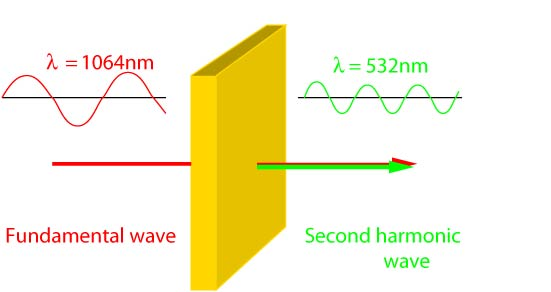
\includegraphics[width = .8\textwidth]{Images/SHG.jpeg}
%  \caption{Depiction of second harmonic generation where an incoming photon, travelling through a nonlinear crystal (yellow block), is converted into two photons, each with half the frequency as the initial photon \protect\cite{SHG}.}
%  \label{fig:SHG}
%\end{figure}

\begin{figure}[ht!]
  \centering
  \includestandalone[width = .8\textwidth]{Images/tikz/shg}
  \caption{Depiction of second harmonic generation where two incoming photons of frequency $f_1$, travelling through a nonlinear crystal, are converted into one photon with frequency $f_2 = 2f_1$, with some light of frequency $f_1$ left over \protect\cite{SHG}.}
  \label{fig:SHG}
\end{figure}
%Birefringence is the property of a material having different refractive indices based upon the polarization of the incoming light; this is unique since for most materials, the index of refraction is uniform and dependent only upon the wavelength of light. For birefringent materials, their exists two different indices of refraction; each of these indices occur when the polarization is parallel to a specific axis within the crystal. These two axes are known as the \textit{ordinary} axis and the \textit{extraordinary} axis; light with polarization along the ordinary axis will follow the standard rules of refraction (hence the name ordinary), given by Equation \ref{snellslaw}. However, light with polarization along the extraordinary axis will travel at a speed different from the light with ordinary polarization due to the difference in the index of refraction the light ``sees'' along each of these axes.

In order to achieve maximum efficiency during a frequency doubling conversion, the phase difference between the fundamental and second harmonic need to be approximately zero, ensuring that no destructive interference occurs. The necessary condition is shown in Fig. \ref{fig:phasematching}, with the wave-vector $\vec{k}$ of the fundamental and second harmonic wave shown. The wave-vector is a vector of magnitude equal to the wavenumber (inverse wavelength) of the wave and direction equal to its propagation direction.



\begin{figure}[h]
  \centering
  \includestandalone{Images/tikz/phasematching}
  \caption{Shown is the phase matching condition of the fundamental and second harmonic wave. In order to achieve maximum efficiency, $\Delta \vec k \approx 0$.}
  \label{fig:phasematching}
\end{figure}

Mathematically, we can define the difference $\Delta \vec k$ between the waves as the sum of the fundamental wave-vector plus twice the second harmonic wave-vector. This relation is

\begin{equation}
  \Delta \vec k = \vec k_1 - 2 \vec k_2,
  \label{phasematching}
\end{equation}
%
where $\vec k_1$ is the wavenumber of the fundamental wave, and $\vec k_2$ is the wavenumber of the second harmonic. Having a difference of $\Delta \vec k = 0$ ensures that no destructive interference between the waves will occur, resulting in maximum output power.

\subsection{Characteristics of the Dye Laser}

The dye laser consisted of a quartz cell filled with fluorescent rhodamine-6G dye dissolved in methanol and a mirror-diffraction grating cavity and was pumped by a Nd:YVO$_4$ solid state laser.

%%%%%%%%%%%%%%%%%%%%%%%%%%%%%%%%%%%%%%%%%%%%%%%%%%
% dyes
%%%%%%%%%%%%%%%%%%%%%%%%%%%%%%%%%%%%%%%%%%%%%%%%%%
When constructing the laser, we used rhodamine-6G as a dye primarily because of its low cost. The rhodamine 6G was dissolved in methanol at an ideal concentration of \SI{0.10}{\gram \per \liter}. Rhodamine 6G, however, does not lase at the wavelength needed for rubidium but instead lases around \SI{566}{\nano \meter}. Once the laser was constructed, we intended to switch to LDS-798, which lases around \SI{785}{\nano \meter}. More information about lasing wavelength, solvents, efficiencies, and concentrations can be found in \textit{Lambdachrome Laser Dyes} \cite{Brackmann2000}.

The dye laser was pumped by a frequency doubled Nd:YVO$_4$ laser with a variable repetition rate from \SI{200}{ kHz} to \SI{4}{ MHz}, a pulse width of \SI{10}{\pico \second}, and wavelength of \SI{1064}{\nano \meter}. The laser produced an average power of around \SI{13}{W} at \SI{200}{\kilo Hz}. The dye solution  absorbs in the visible range, not the infrared, which created the necessity for frequency doubling.

When using a frequency doubling crystal, it is important to maintain the alignment and temperature of the crystal, since both of these can impact the performance of the second harmonic generation process. The temperature of the crystal was controlled using a transistor-thermistor combination. The transistor controlled whether current flowed through the crystal housing. If current did flow, the transistor would heat up, in turn heating up the crystal. The temperature of the crystal was monitored using a thermistor, a resistor whose resistance changes with temperature. 

In order to accurately monitor the temperature, the thermistor needs to be calibrated. This was done by allowing current to pass through the transistor and measuring the resistance of the thermistor at various temperatures (measured with a mercury thermometer). The data used for this calibration are shown in Fig. \ref{fig:rvt}. It was found that the temperature followed the function

\begin{equation}
	T = (-0.21 \pm 0.01)  R + (117.74 \pm 1.28),
	\label{eq:RvT}
\end{equation}
%
where $R$ is the resistance in Ohms and $T$ is the temperature in degrees Celsius. This allowed the temperature of the crystal to be measured by simply measuring the resistance of the thermistor.


%%%%%%%%%%%%%%%%%%%%%%%%%%%%%%%%%%%%%%%%%%%%%%%%%%
% Figure of temperature versus resistance for thermistor
%%%%%%%%%%%%%%%%%%%%%%%%%%%%%%%%%%%%%%%%%%%%%%%%%%
\begin{figure}[h]
  \centering
  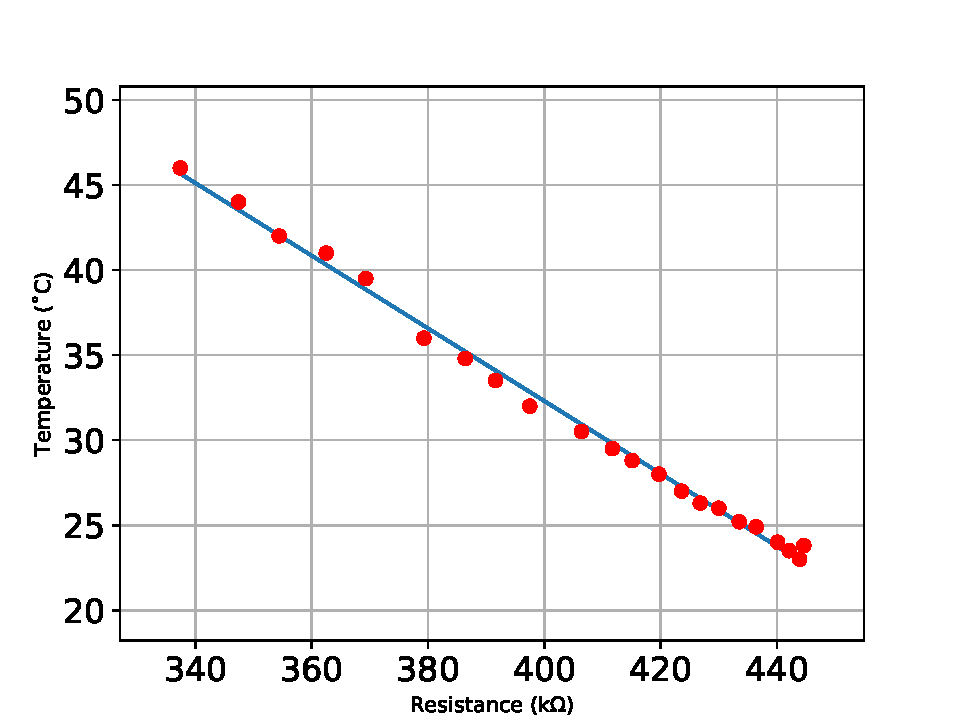
\includegraphics[width = .8\textwidth]{Images/bestfitRvT.pdf}
  \caption{Temperature of the thermistor as a function of its resistance. A linear best fit function is plotted, given by Eq. \ref{eq:RvT}.}
  \label{fig:rvt}
\end{figure}


The temperature of the crystal was also measured as a function of the current through the transistor. A specific current was supplied to the transistor, two minutes were allotted for the crystal to heat up, and the temperature was then measured with a mercury thermometer. A figure of these data is shown in Fig. \ref{fig:tvsi}, and the temperature is shown to increase rapidly as current increases.

%%%%%%%%%%%%%%%%%%%%%%%%%%%%%%%%%%%%%%%%%%%%%%%%%%
% Temperature versus current
%%%%%%%%%%%%%%%%%%%%%%%%%%%%%%%%%%%%%%%%%%%%%%%%%%
\begin{figure}[h!]
  \centering
  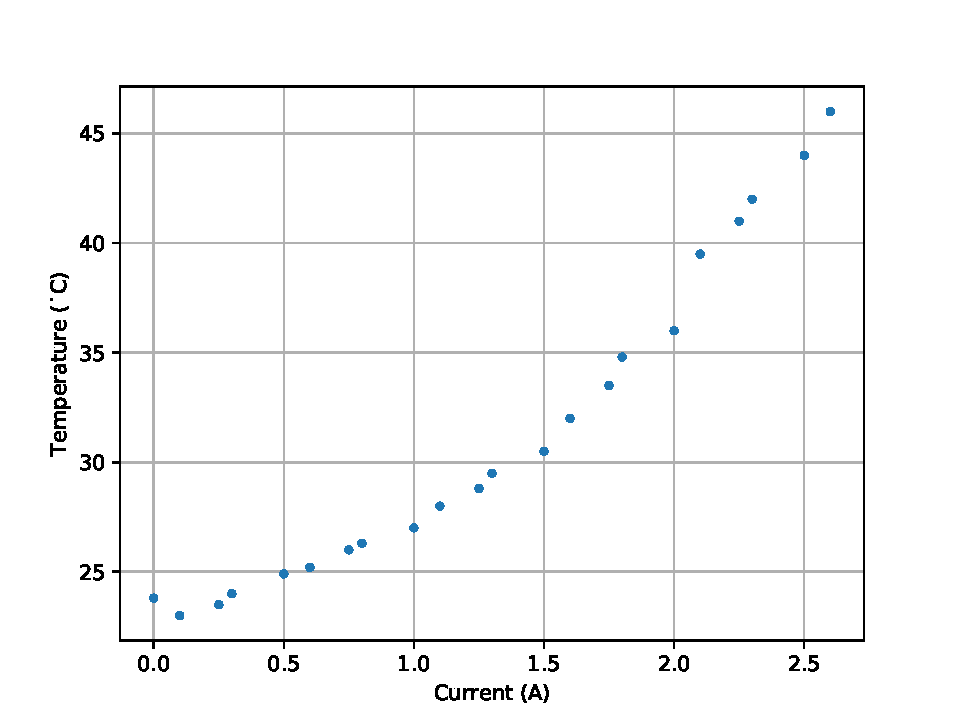
\includegraphics[width = .8\textwidth]{Images/TvsI.pdf}
  \caption{Graph of the temperature of the crystal plotted versus current through the transistor.}
  \label{fig:tvsi}
\end{figure}


Two times series were also taken of the resistance of the thermistor and the temperature of the crystal. These were both measured by running \SI{5}{ A} of current through the transistor. The resistance decreases rapidly over time with very small fluctuations in resistance, as shown in Fig. \ref{fig:resfluct}. The temperature increases exponentially in time with small fluctuations, especially at higher temperatures. These fluctuations, however, may simply be an artifact of the thermometer as opposed to actual temperature fluctuations in the crystal. The temperature versus time data are shown in Fig. \ref{fig:tempflucfit}, along with an exponential best fit for the temperature data, given by

\begin{equation}
	T = 47.7 - 22.7 e^{-t/308.7},
	\label{eq:temptime}
\end{equation}
%
where $T$ is the temperature in degrees Celsius and $t$ is time in seconds.


%%%%%%%%%%%%%%%%%%%%%%%%%%%%%%%%%%%%%%%%%%%%%%%%%%
% Resistance versus times
%%%%%%%%%%%%%%%%%%%%%%%%%%%%%%%%%%%%%%%%%%%%%%%%%%
\begin{figure}[h!]
  \centering
  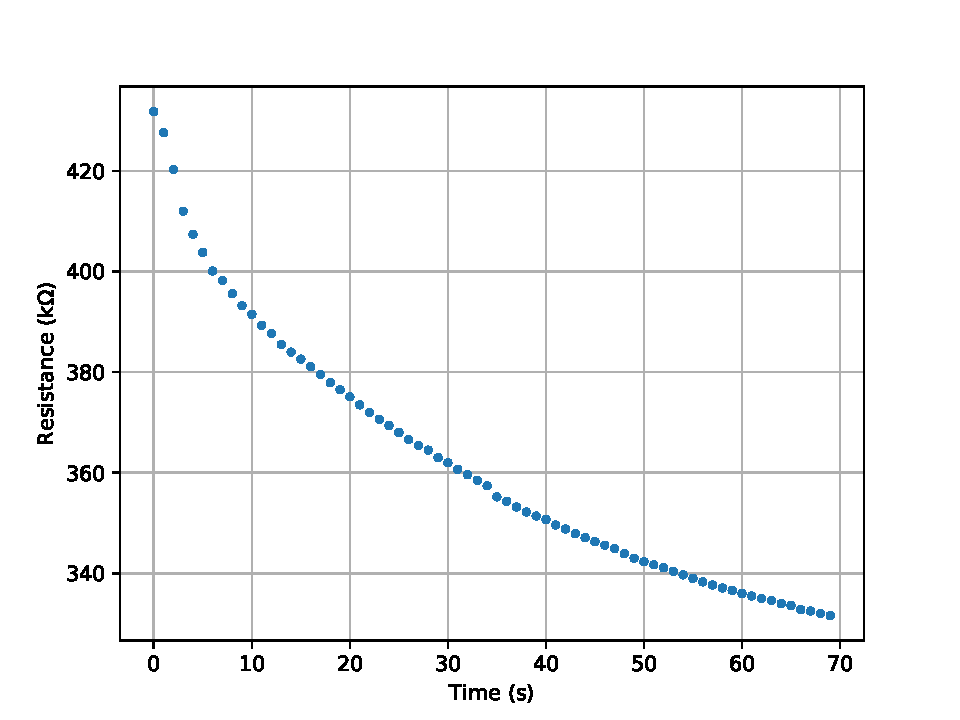
\includegraphics[width = .8\textwidth]{Images/ResFluct.pdf}
  \caption{Graph of the change in resistance of the thermistor over time at fixed current of \SI{5}{ A}.}
  \label{fig:resfluct}
\end{figure}
%%%%%%%%%%%%%%%%%%%%%%%%%%%%%%%%%%%%%%%%%%%%%%%%%%
% Temperature versus time
%%%%%%%%%%%%%%%%%%%%%%%%%%%%%%%%%%%%%%%%%%%%%%%%%%
\begin{figure}[h!]
  \centering
  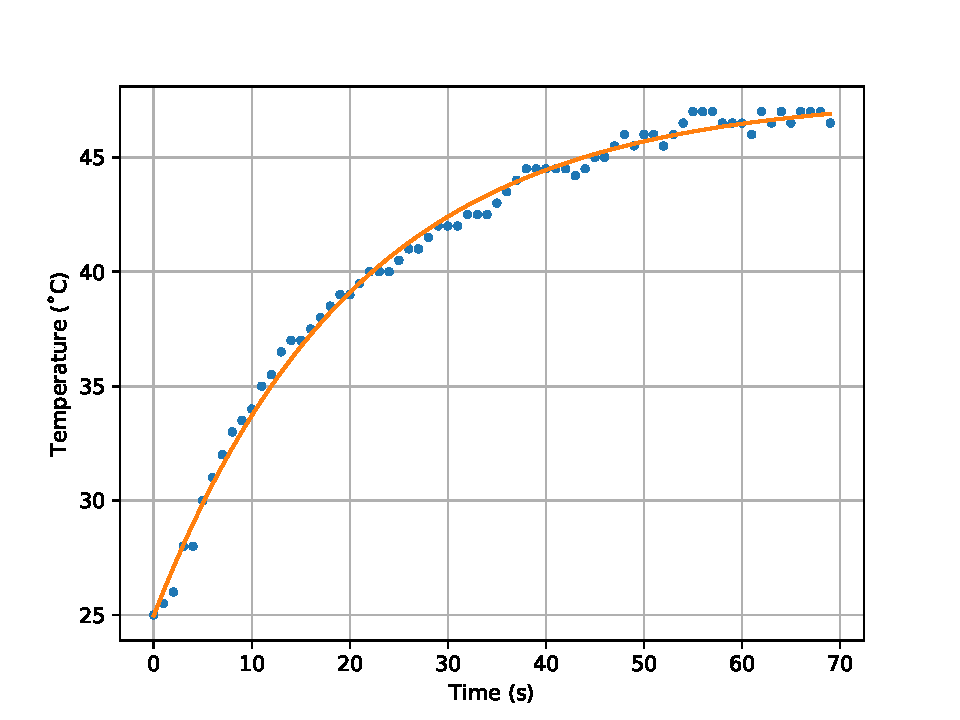
\includegraphics[width = .8\textwidth]{Images/TempFluctFit.pdf}
  \caption{Graph of the change in temperature as a function of time at fixed current of \SI{5}{ A}. An exponential best fit is plotted on top of these data, given by Eq. \ref{eq:temptime}.}
  \label{fig:tempflucfit}
\end{figure}

The crystal, transistor, and thermistor were found to function according to expectations, and were thus ready to be used for second harmonic generation. Using a spectrometer to measure the wavelength of light transmitted through the crystal, the crystal was aligned for optimal conversion of \SI{1064}{\nano \meter} light into \SI{532}{\nano \meter} light. This was done with \SI{5}{ A} of current running through the transistor in order to heat the crystal. A figure of the spectrum at poor alignment is shown in the left panel of Fig. \ref{fig:conversionspectrum1}, where the peak on the left is the amount of \SI{532}{\nano \meter} light transmitted and the peak on the right is the amount of \SI{1064}{\nano \meter} light transmitted through the crystal. It can be seen that only a small fraction of the fundamental light is converted into the second harmonic light. The crystal was most sensitive to rotations about the axis perpendicular to the optical axis, but its efficiency depended also upon vertical and horizontal adjustments. At optimal alignment, the crystal converted roughly 65\% of the initial \SI{1064}{\nano \meter} light into \SI{532}{\nano \meter} light. This can be seen in the right panel of Fig. \ref{fig:conversionspectrum1}, where more \SI{532}{\nano \meter} light is seen than \SI{1062}{\nano \meter} light. Typically, conversion efficiencies (amount of \SI{532}{\nano \meter} light divided by the amount of \SI{532}{\nano \meter} plus \SI{1064}{\nano \meter} light) above 50\% are expected and around 70\% to 80\% are good. For our purposes, 65\% was sufficient.

%%%%%%%%%%%%%%%%%%%%%%%%%%%%%%%%%%%%%%%%%%%%%%%%%%
% Figure of spectrum of crystal
%%%%%%%%%%%%%%%%%%%%%%%%%%%%%%%%%%%%%%%%%%%%%%%%%%
\begin{figure}[h!]
  \centering
  \begin{minipage}{.45\textwidth}
	  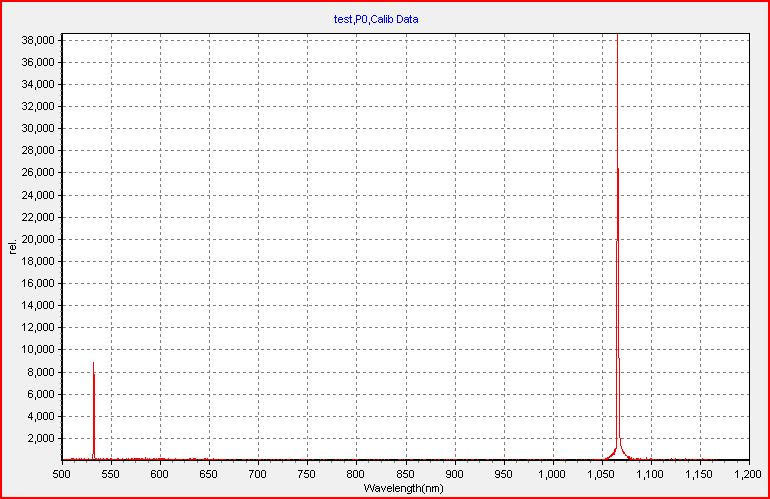
\includegraphics[scale = .32]{Images/doublingCrystalWright2017.JPG}
  \end{minipage}
  \begin{minipage}{.45\textwidth}
	  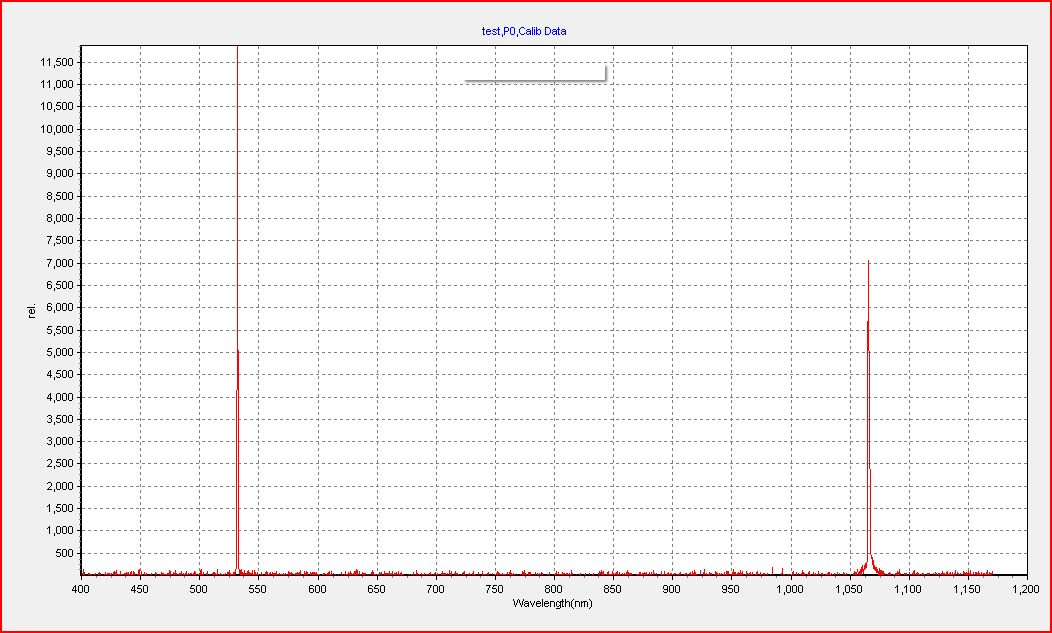
\includegraphics[scale = .25]{Images/goodspectrum.JPG}
  \end{minipage}
  \caption{Spectrum of converted laser light through doubling crystal before alignment (left) and after alignment (right). \SI{532}{\nano \meter} light shown on the left peak and \SI{1064}{\nano \meter} light shown on the right peak.}
  \label{fig:conversionspectrum1}
\end{figure}

With spatial alignment optimized, the conversion efficiency also needed to be optimized with respect to the temperature of the crystal. In optimal spatial alignment, at maximum temperature (current at \SI{5}{ A}), the current was turned off and the conversion efficiency was measured at various resistances. Since resistance depends upon temperature, this gives a measurement of efficiency versus temperature. These data are shown in Fig. \ref{fig:crystaleff}, and the efficiency clearly decreases with increasing resistance. Since temperature decreases with increasing resistance, it was decided that in order to convert the maximum amount of \SI{532}{\nano \meter} light, the temperature needed to be increased. However, even with temperatures above the previously mentioned test, the conversion efficiency never exceeded the previously measured 65\%. This efficiency turned out to be the maximum conversion efficiency. Any deviations from it were simply misalignments as the temperature changed. For all temperatures, the 65\% efficiency could be established through spatial re-alignment. Thus, since the conversion efficiency was not dependent upon the temperature of the crystal but only upon spatial alignment, we did not stabilize the temperature of the crystal.

With the medium and pump of the dye laser constructed, the cavity needed to be constructed and aligned. The final cavity would consist of a silver coated mirror on one end and a diffraction grating on the other, schematically shown in Fig. \ref{fig:dyelaser}. However, for initial alignment, it is easiest to replace the diffraction grating with a glass slide acting as a partially transmissive mirror. The cavity was initially aligned by pumping the medium with a \SI{532}{\nano \meter} Nd:YAG solid state laser, with a repetition rate of \SI{10}{ Hz} and a pulse width on the order of \SI{10}{\nano \second}. This made initial alignments much easier due to the longer pulse width of the Nd:YAG laser. After the cavity was lasing through excitation with the Nd:YAG laser, the Nd:YAG was turned off and the Nd:YVO$_4$ was switched on. The cavity was then realigned through excitation in an attempt to ellicit lasing from the Nd:YVO$_4$. However, no lasing was ever seen. Power meters, photodiodes, and spectrometers were employed to search for small amounts of lasing light from the cavity but yielded no results. It was concluded that the pulse width of the pump beam was indeed too short for our cavity to lase, and the dye laser was abandoned.

It should be noted that a superposition of lasers beams was also attempted. It was thought that small amounts of stimulated emission could be produced with the longer pulse Nd:YAG, and then, by overlapping the Nd:YVO$_4$ beam with the Nd:YAG beam, the dye laser could be pushed over the threshold and begin lasing. There are various problems with this (e.g. beating), but regardless, lasing was still not established.

%%%%%%%%%%%%%%%%%%%%%%%%%%%%%%%%%%%%%%%%%%%%%%%%%%
% Figure of the efficiency of the crystal
%%%%%%%%%%%%%%%%%%%%%%%%%%%%%%%%%%%%%%%%%%%%%%%%%%
\begin{figure}[h!]
  \centering
  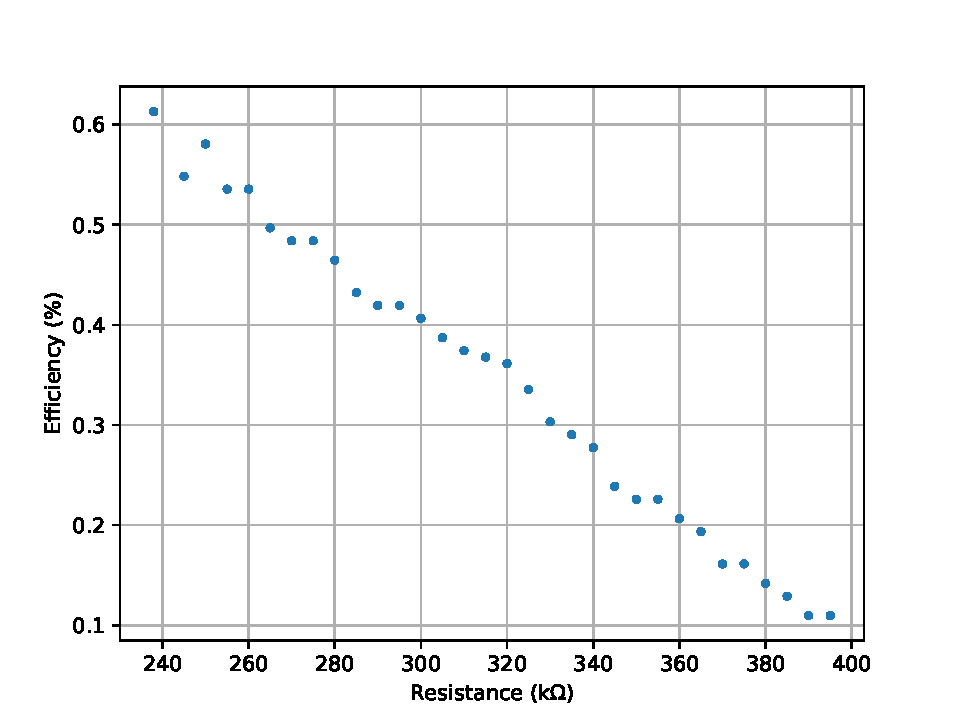
\includegraphics[width = .8\textwidth]{Images/efficiency.pdf}
  \caption{Efficiency of the doubling crystal versus the resistance (and thus temperature) of the crystal. This, however, is simply an artifact of changes in alignment of the crystal as the temperature changes.}
  \label{fig:crystaleff}
\end{figure}






%%%%%%%%%%%%%%%%%%%%%%%%%%%%%%%%%%%%%%%%%%%%%%%%%%
% Diode Laser
%%%%%%%%%%%%%%%%%%%%%%%%%%%%%%%%%%%%%%%%%%%%%%%%%%
\section{Diode Lasers and Acousto-Optic Modulators}

In addition to investigating the use of dye lasers as an MRP laser system, we also investigated the use of a diode laser, pulsed by chopping the beam with an acousto-optic modulator (AOM). This system was able to produce the required criteria for a MRP laser.

\subsection{Laser Diodes}
A laser diode is a semiconductor device that makes use of a p-n junction to produce stimulated emission. This p-n junction consists of two semiconductors placed side by side, one p-doped and the n-doped. P-doping inserts atoms that contain one or two electrons less than the atoms in the semiconductor have. N-doping places atoms with one or two more electrons than the atoms in the semiconductor. This makes the p-doped semiconductor ``positive'' with ``holes'' for electrons in the ``negative'' n-doped semiconductor to transition into. If a potential difference is supplied across this junction, electrons from the n-doped semiconductor are pushed towards the p-doped semiconductor. This situation then allows for electrons to decay into the ``holes'' provided by the p-donors, emitting a photon upon decay. The semiconductor is typically highly polished and thus acts as its own cavity.


The wavelength of light emitted from laser diodes is dependent upon the material of the semiconductor. Many different diode lasers are available with various wavelengths, including $\SI{780}{\nano\meter}$ for the rubidium absorption. Typically, laser diodes have a linewidth of a few nanometers, but a specific wavelength of light can be selected from this linewidth with a method similar to that of the dye laser. Using a diffraction grating, light from the diode laser can be spread out and reflected back into the laser diode. The particular wavelength reflected back into the diode will stimulate the emission of photons of a similar wavelength, thereby narrowing the overall linewidth of the laser.

Diode lasers are, however, continuous wave lasers. In order to make a \textit{pulsed} diode laser, we use an acousto-optic modulator (AOM), a device that makes use of the propagation of sound waves through a crystal to diffract light. A schematic of an AOM is shown in Fig. \ref{fig:AOM1}. A crystal is attached to a piezo-electric transducer (PZT) that can be driven by an electric signal. When a signal is supplied to the PZT, oscillations are produced that propagate through the crystal in a periodic manner. These  compressions in the crystal act similar to sound waves travelling through a solid. These waves cause a periodic change in the index of refraction, causing incident light to diffract,\footnote{This process can also be described by particles instead of waves. The sound waves can be quantized and thought of as discrete particles, known as phonons. As light enters the crystal perpendicular to the propagation direction of the phonons, the photons will collide with the phonons, and by conservation of momentum, be deflected. This creates a ``diffracted'' beam.} similar to a traditional diffraction grating.

%\begin{figure}[h]
%		\centering
%		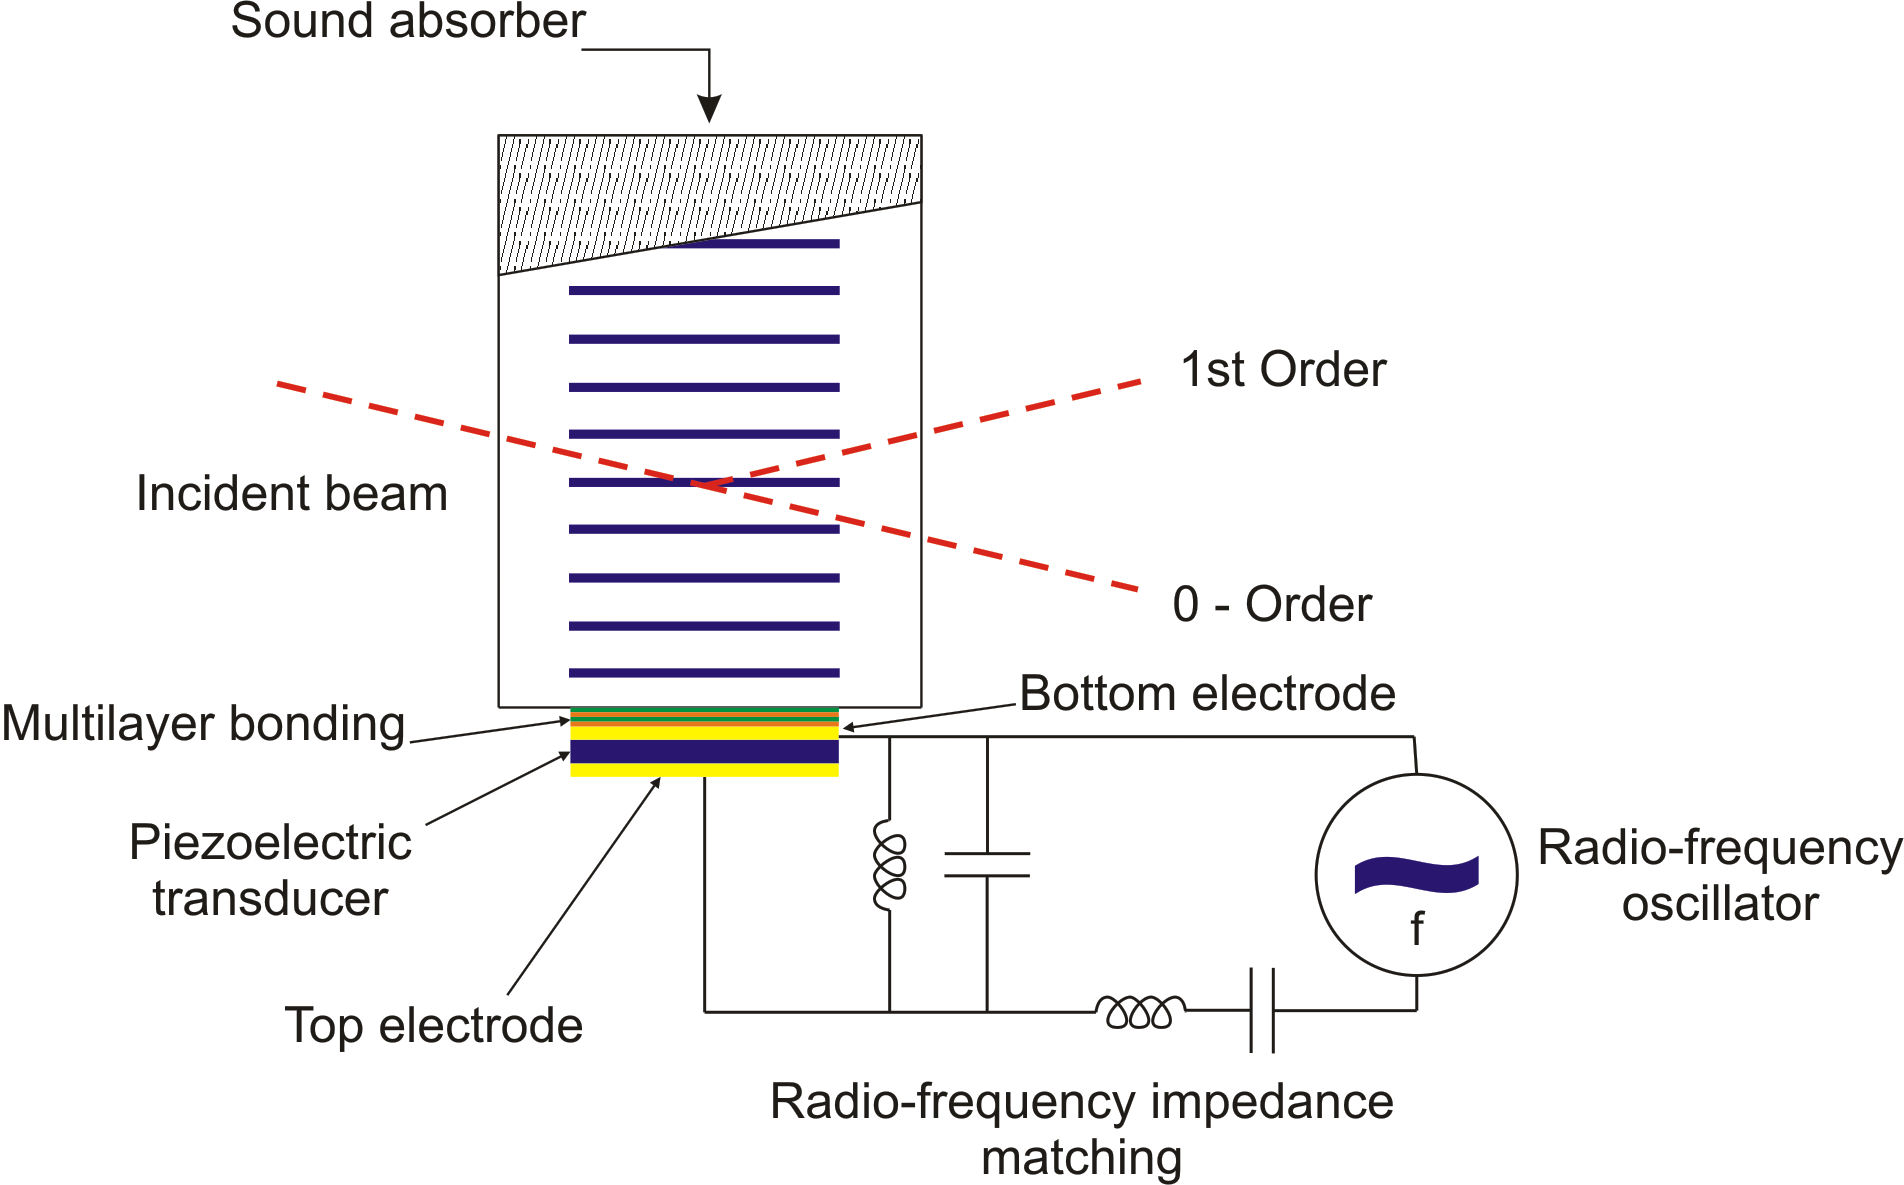
\includegraphics[width = .8\textwidth]{Images/AOM1.png}
%		\caption{Schematic of an acousto-optic modulator. The dashed red line is the laser beam coming from left to right that is diffracted by the AOM into a first and second order beam \protect\cite{aomfig}.}
%		\label{fig:AOM1}
%\end{figure}

\begin{figure}[h]
		\centering
		\includestandalone[width = .8\textwidth]{Images/tikz/aom}
		\caption{Schematic of an acousto-optic modulator. The beam on the left is the laser beam coming from left to right that is diffracted by the AOM into a first and second order beam \protect\cite{aomfig}.}
		\label{fig:AOM1}
\end{figure}

If we take the first order beam to be our laser beam, we can create a pulsed laser simply by turning on and off the PZT. When the PZT is turned on, it will diffract the incoming beam, creating a pulse of light, and when it is turned off, the incoming beam will no longer be diffracted and the pulse will be cut off. Thus, the length of time the PZT is turned on for will determine the pulse width of our laser, and the frequency at which we turn the PZT on and off will determine the repetition rate of the laser.


\subsection{Characterization of the Diode Laser}

The diode laser was constructed using a continuous wave, \SI{780}{\nano \meter} laser diode. The laser is kept on resonance with the rubidium D$_2$ line using a continuously scanning diffraction grating. The diffraction grating separates out light into its various frequencies and reflects one of these frequencies of light back into the laser diode. With a piezo-electric transducer (PZT), the angle of the diffraction grating is continuously varied in an oscillating manner, allowing the laser to scan over a small range of wavelengths. This allows wavelengths around the resonant frequency to be reflected back into the diode, which stimulates the emission of more photons of this wavelength. By sending part of this laser light through a rubidium cell and measuring its absorption, the PZT can be tuned such that maximum light is absorbed in the rubidium cell. The PZT is continuously scanning during operation, allowing for precise tuning of the wavelength to the rubidium D$_2$ line.

As mentioned earlier, the diode laser was pulsed, or ``chopped,'' with an AOM. The AOM was driven with a voltage from a function generator (Agilent 33120A) capable of producing step function voltages with repetition rates up to \SI{15}{\mega \hertz} and a duty cycle greater than or equal to 20\%. The function generator and AOM pulsed the diode laser beam as expected. With a 20\% duty cycle and a repetition rate of \SI{250}{ kHz}, the pulses appeared very square (as measured on an oscilloscope with a photodiode, shown in Fig. \ref{fig:diodepulse1}). The under and overshoots seen at the beginning and end of the pulses is likely just an artifact of imprecise electronic behavior of the photodiode at such short timescales. The diode laser light is originally linearly polarized. This linearly polarized light is filtered into horizontally polarized light with a half-waveplate and a polarizing beam splitting cube. This allowed adjustment of the intensity by rotation of the waveplate. Finally, the light is converted into $\sigma ^+$ circularly polarized light with a quarter-waveplate in order to optically pump the rubidium.

The laser could thus be operated in pulsed mode by applying a periodic voltage to the AOM or could be operated in continuous mode by applying a constant voltage to AOM. The laser had an maximum average power of \SI{2}{\milli W} when operating in pulsed mode with repetition rates in the hundreds of kilohertz, and an maximum average power of \SI{5}{\milli W} when operating in continuous mode. The laser beam had a radius on the order of \SI{2}{\milli \meter}, giving an intensity of around \SI{100}{W \per \meter \squared} in pulsed mode and \SI{400}{W \per \meter \squared} in continuous mode.

%%%%%%%%%%%%%%%%%%%%%%%%%%%%%%%%%%%%%%%%%%%%%%%%%%
% diode pulses
%%%%%%%%%%%%%%%%%%%%%%%%%%%%%%%%%%%%%%%%%%%%%%%%%%
\begin{figure}[ht!]
		\centering
		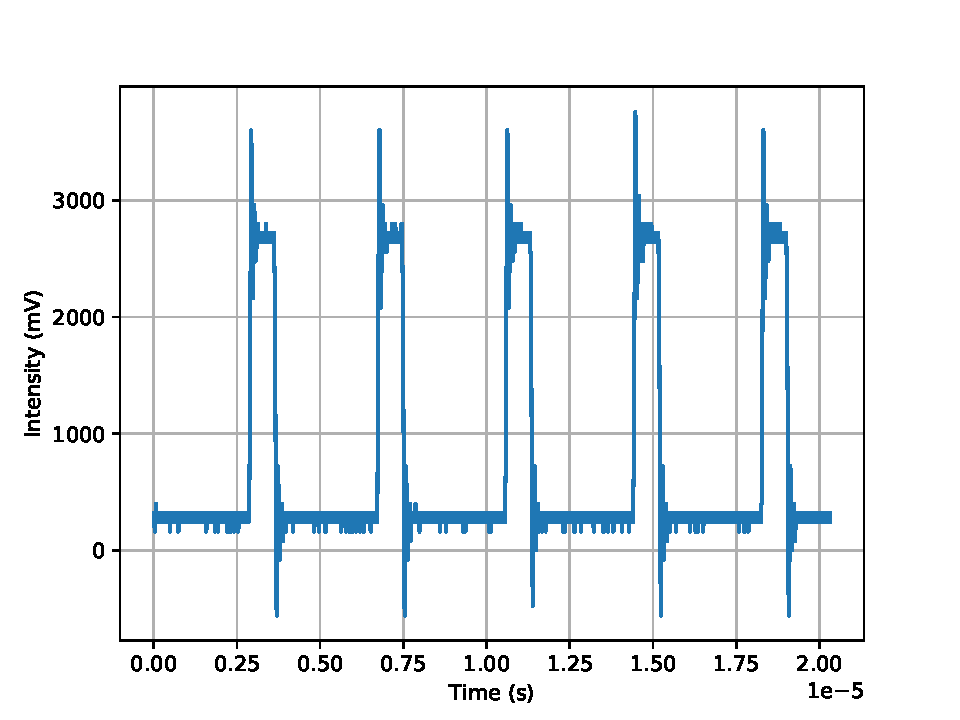
\includegraphics[width = .8\textwidth]{Images/diodepulse.pdf}
		\caption{Shown are the laser pulses from the diode laser pulsed with an AOM taken on an oscilloscope. The pulses have a repetition rate of \SI{250}{ kHz} and a duty cycle of 20\%.}
		\label{fig:diodepulse1}
\end{figure}

%\begin{figure}[h]
%		\centering
%		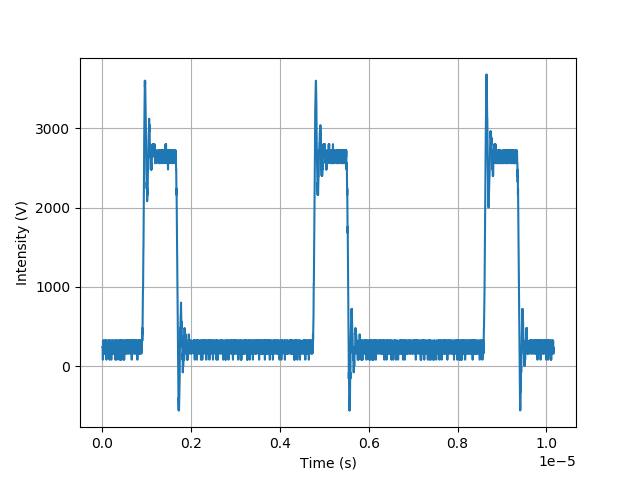
\includegraphics[scale=0.5]{Images/diodepulse2.png}
%		\caption{Figure of a zoomed in image of the diode pulse.}
%		\label{fig:diodepulse2}
%\end{figure}

An important aspect of the diode-AOM system is the rise and fall time. These are the times that each laser pulse takes to reach its maximum and minimum amplitude respectively. Essentially, it is how quickly the AOM can diffract the laser beam. Ideally, both of these times would be as short as possible, creating a highly square wave, similar to a step function. However, due the physical width of the laser beam, there will be some time over which only part of the beam is diffracted (as the ``sound waves'' travel through the crystal and interact with the laser beam). Thus, having a tightly focused narrow beam will decrease both the rise and fall times. A converging lens was placed before the AOM and was adjusted to minimize the rise and fall times of the pulse. The pulses had a rise time on the order of \SI{10}{\nano \second}, which is great for a laser with a pulse width on the order of microseconds. 

In conclusion, we constructed a pulsed diode laser that satisfied the necessary criteria for a MRP laser. The diode laser was on resonance with the rubidium D$_2$ line, had a variable repetition rate controlled with a function generator, and had a low duty cycle of 20\%. Furthermore, its polarization could be manipulated with half- and quarter-waveplates and polarizing beam splitting cubes.

%%%%%%%%%%%%%%%%%%%%%%%%%%%%%%%%%%%%%%%%%%%%%%%%%%
% Magnetic Field
%%%%%%%%%%%%%%%%%%%%%%%%%%%%%%%%%%%%%%%%%%%%%%%%%%
\chapter{Magnetic Field Housing}


In order to model the magnetic field environment that laser guide star systems encounter, a configurable magnetic field needed to be constructed. This magnetic field needed to be variable in its strength, be spatially homogeneous in strength, and be able to be rotated in order to create an angle between field direction and the laser beam. This chapter describes and characterizes this magnetic field configuration.

A homogeneous magnetic field of strength 0 - \SI{10}{Gauss} was created using a Helmholtz coil configuration.\footnote{This magnetic field could have been created much more simply using magnetic monopoles, but unfortunately they are hard to get your hands on. Some people still even insist $\vec \nabla \cdot \vec B = 0$.} A schematic of the Helmholtz coils is shown in Fig. \ref{fig:helmholtzcoils} and a photograph of the setup is shown in Fig. \ref{fig:actualcoils}. The coils have an inner radius of \SI{10}{\centi \meter}, an outer radius of \SI{12}{\centi \meter}, a width of \SI{1}{\centi \meter}, and are separated by a distance of \SI{10}{\centi \meter}. Each coil has 155 turns, with approximately 10 turns along the axial direction and 15 layers of coil in the radial direction. The coils were connected with a metal rod attached to the botton of each coil. The center of the rod contained a hole which screwed into the optical table, allowing for rotation of the coils (and thus of the magnetic field) about an axis perpendicular to the laser beam. This allowed for direct manipulation of the angle of the magnetic field with respect to the laser beam. Current was supplied with a standard DC power supply through the coils. The wiring of the coils was 20 AWG gauge, which is limited to a current of \SI{1.5}{ A}.

\begin{figure}[htpb]
	\centering
	\includestandalone{Images/tikz/magfield}
	\caption{Schematic of the Helmholtz coil configuration used for the main magnetic field in this experiment.}
	\label{fig:helmholtzcoils}
\end{figure}



\begin{figure}[htpb]
	\centering
	\begin{tikzpicture}
	\node at (0,0) {\includegraphics[width=0.8\textwidth]{Images/actualcoils.png}};
	\node[text = white] at (-4,-3.5) {\large Compensation};
	\node[text = white] at (-4,-4) {\large Coils};

	\node[text = white] at (0,-2.7) {\large Main};
	\node[text = white] at (0,-3.2) {\large Coils};

	\draw[red, line width = 1.6pt] (-3.5,-.5) -- (-1.5,-.5);
	\draw[red,->,>=stealth, line width = 1.6pt] (1.65,-.5) -- (3.75,-.5);
	\node[text = white] at (2.5,-1) {\large Laser};
	\node[text = white] at (2.5,-1.5) {\large Beam};

	\node[text = white] at (-1.5,2) {\large Photodiode};
	\end{tikzpicture}
	\caption{Main coils (inside, black) shown along with the compensation coils (outside, blue).}
	\label{fig:actualcoils}
\end{figure}

The expected magnetic field strength along the axial direction and along the radial direction were computationally calculated. These data are shown in Fig. \ref{fig:axialtheoretical}. For a current of \SI{1}{ A}, the expected magnetic field was nearly \SI{13}{ G}, which is more than sufficient for our purposes. Furthermore, the calculation showed a homogeneity of \SI{\pm 0.1}{ Gauss} in the axial direction and of \SI{\pm 0.2}{ Gauss} in the radial direction. These two calculations confirmed that this Helmholtz configuration would supply the necessary magnetic field.

\begin{figure}[htpb]
	\centering
	\begin{minipage}{.49\textwidth}
	\centering
	\begin{tikzpicture}
		\node at (0,0) {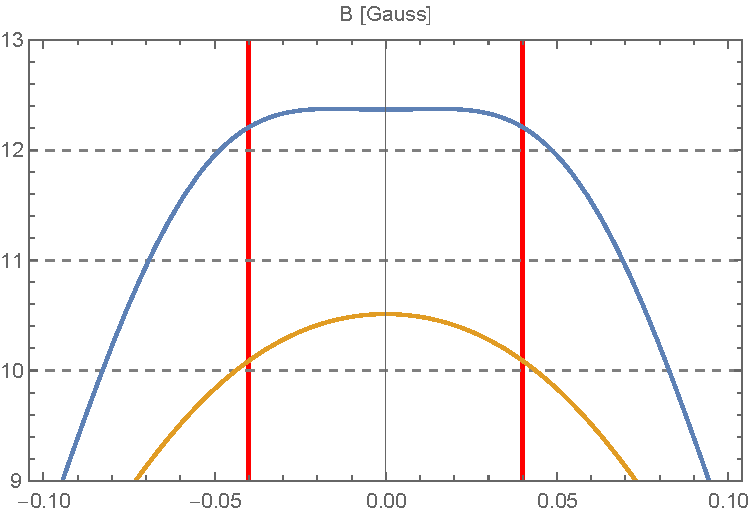
\includegraphics[width=0.9\textwidth]{../../Helmholtz/axialtheoretical.pdf}};
		\draw[fill = white,white] (-1,2) rectangle (1,2.5);
		\node[rotate = 90] at (-3.5,0) {\scriptsize Magnetic Field (Gauss)}; 
		\node[] at (0,-2.5) {\scriptsize Axial Distance from Center (m)}; 
	\end{tikzpicture}
	\end{minipage}
	\begin{minipage}{.49\textwidth}
	\centering
	\vspace{.5cm}
	\begin{tikzpicture}
		\node at (0,0) {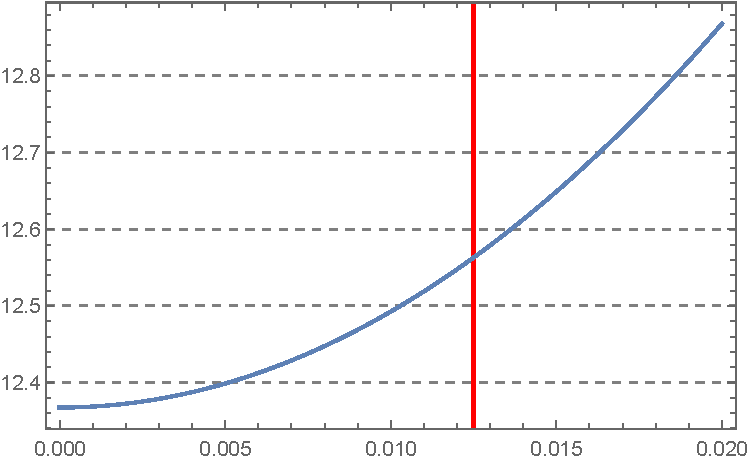
\includegraphics[width=0.9\textwidth]{../../Helmholtz/radialtheoretical.pdf}};
		\node[rotate = 90] at (-3.5,0) {\scriptsize Magnetic Field (Gauss)}; 
		\node[] at (0,-2.5) {\scriptsize Radial Distance from Center (m)}; 
	\end{tikzpicture}
	\end{minipage}
	\caption{Numerical results for the field strength along the axial and radial direction for our Helmholtz configuration (blue) and a Helmholtz configuration with a longer distance between coils than radius of coils (yellow). The axial and radial dimensions of the rubidium cell are shown in red. Simulation by Dr. Michaela Kleinert.}
	\label{fig:axialtheoretical}
\end{figure}


The support structure was 3D printed in Dr. Daniel Borrero's lab and the wiring was coiled by hand. The strength and homogeneity of the magnetic field was measured with a Gauss meter. The configuration performed as expected, producing a homogeneous magnetic field in both the radial and axial direction. In the axial direction in between the coils, the magnetic field stayed within \SI{\pm 0.25}{ G} for a current of \SI{0.5}{ A} and within \SI{\pm 0.5}{ G} for a current of \SI{1.0}{ A}. A graph of these data is shown in Fig. \ref{fig:FieldAxial} with vertical lines showing the boundary of the coils. In the radial direction for both \SI{0.5}{ A} and \SI{1.0}{ A}, the magnetic field stayed with \SI{\pm 0.25}{ G} for a radius less than \SI{7}{\centi \meter}. Beyond this this radius, the magnetic field decreased significantly. A graph of the radial magnetic field is shown in Fig. \ref{fig:FieldRadial}, with vertical lines showing the boundary of the coils. The rubidium cell, being \SI{8}{\centi \meter} long and having a diameter of \SI{1.0}{\centi \meter}, is well within the range of homogeneity.



%%%%%%%%%%%%%%%%%%%%%%%%%%%%%%%%%%%%%%%%%%%%%%%%%%
% Axial Magnetic Field
%%%%%%%%%%%%%%%%%%%%%%%%%%%%%%%%%%%%%%%%%%%%%%%%%%
\begin{figure}[h]
		\centering
		\begin{minipage}{.49\textwidth}
			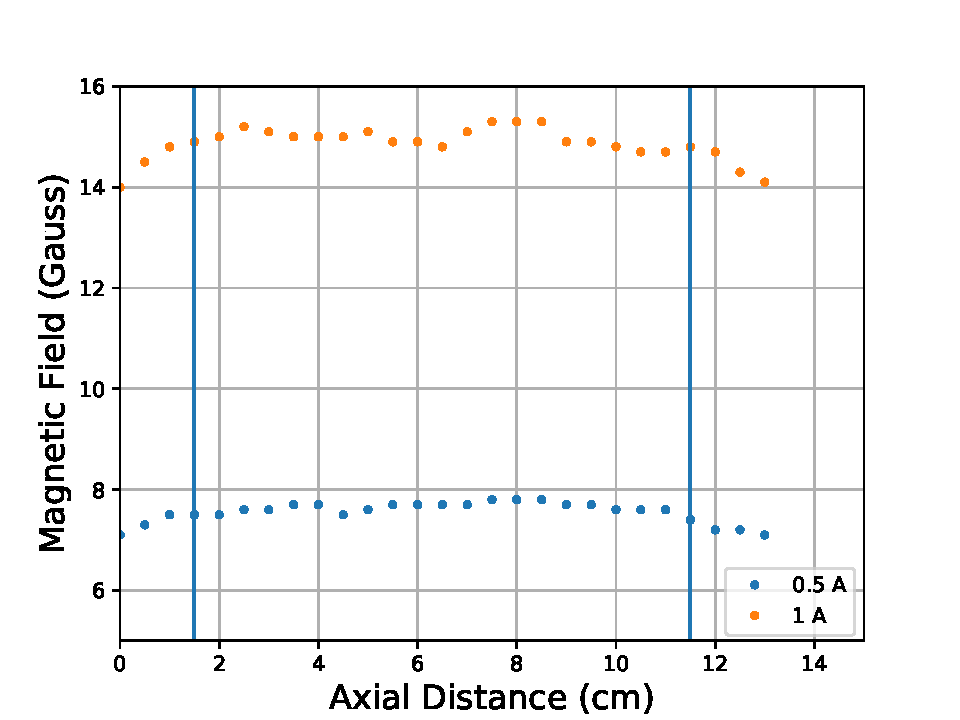
\includegraphics[width = .9\textwidth]{Images/FieldAxial.pdf}
		\end{minipage}
		\begin{minipage}{.49\textwidth}
			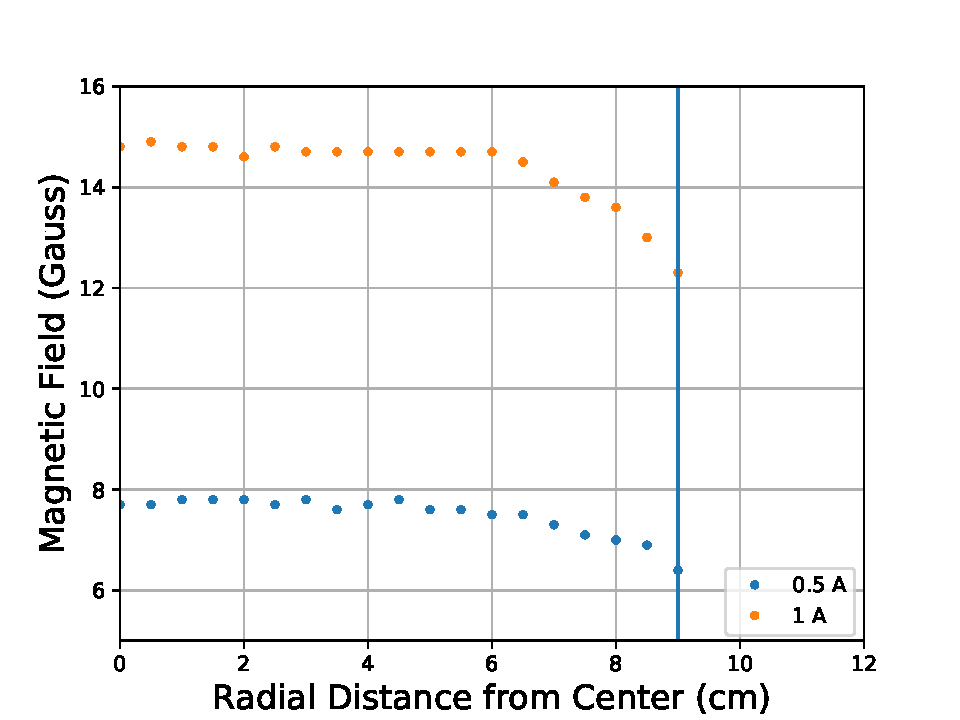
\includegraphics[width = .9\textwidth]{Images/FieldRadial.pdf}
		\end{minipage}
		\caption{Graph of the magnetic field along the axial and radial direction for currents of \SI{1.0}{A} and \SI{0.5}{A}.}
		\label{fig:FieldAxial}
\end{figure}

%%%%%%%%%%%%%%%%%%%%%%%%%%%%%%%%%%%%%%%%%%%%%%%%%%
% Radial Magnetic Field
%%%%%%%%%%%%%%%%%%%%%%%%%%%%%%%%%%%%%%%%%%%%%%%%%%
\begin{figure}[h!]
		\centering
		\caption{Graph of the magnetic field along the radial direction for currents at \SI{1.0}{A} and \SI{0.5}{A}.}
		\label{fig:FieldRadial}
\end{figure}

The strength of the magnetic field was measured at the center of the coils as a function of the current through the coils. This allowed a direct calculation of the magnetic field, knowing only the current being supplied to the coils. These data are shown in Fig. \ref{fig:FieldvCurrent} along with a line of best fit. As expected, the relationship between magnetic field strength and current is linear, given by

\begin{equation}
	B = 13.23 I-0.28,
	\label{eq:fieldvcurrent}
\end{equation}
%
where $B$ is the magnetic field in Gauss and $I$ is the current in amperes.

%%%%%%%%%%%%%%%%%%%%%%%%%%%%%%%%%%%%%%%%%%%%%%%%%%
% Field versus current
%%%%%%%%%%%%%%%%%%%%%%%%%%%%%%%%%%%%%%%%%%%%%%%%%%
\begin{figure}[h]
		\centering
		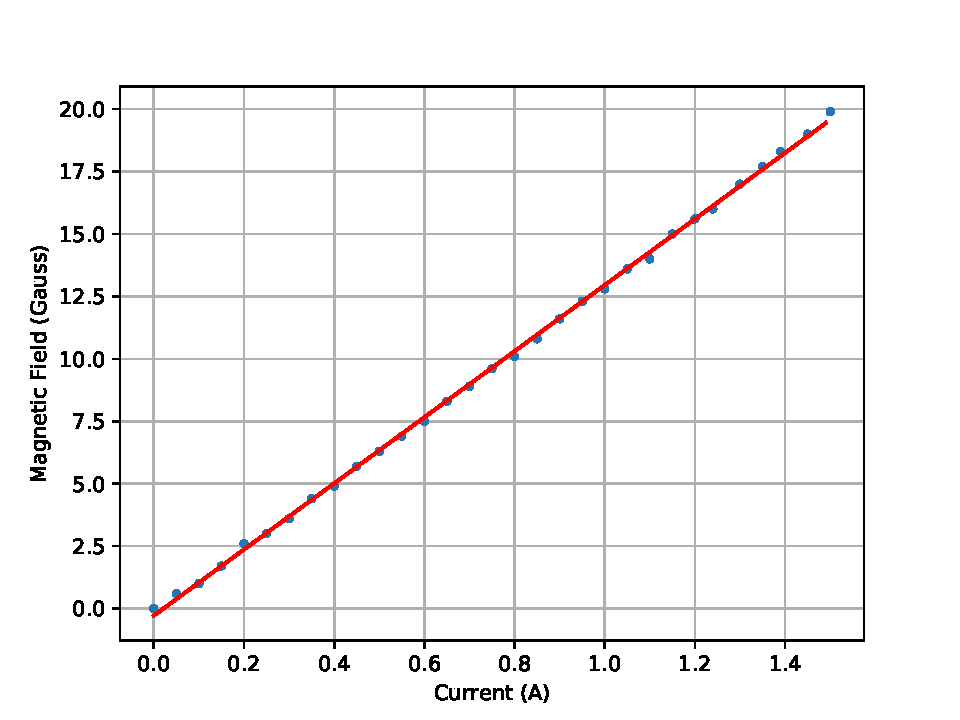
\includegraphics[width = .8\textwidth]{Images/FieldvCurrent.pdf}
		\caption{Graph of the strength of the magnetic field in the center of the Helmholtz coils as a function of current.}
		\label{fig:FieldvCurrent}
\end{figure}

In addition to the coils described above, which we will call the main coils, a second pair of Helmholtz coils was used to compensate for the geomagnetic field and other stray magnetic fields in the lab. These coils, which we will call the compensation coils, were placed outside of the main coils and oriented in the direction of the geomagnetic field. The compensation coils are shown in blue steel housing and copper wiring in Fig. \ref{fig:actualcoils}. They created a homogeneous magnetic field equal and opposite to the geomagnetic field so that the only magnetic field in the experiment was from the main coils.



%%%%%%%%%%%%%%%%%%%%%%%%%%%%%%%%%%%%%%%%%%%%%%%%%%
% Fluorescence Measurements
%%%%%%%%%%%%%%%%%%%%%%%%%%%%%%%%%%%%%%%%%%%%%%%%%%
\chapter{Fluorescence Measurements}
With a laser on resonance with rubidium and capable of being pulsed or continuous wave, a magnetic field of variable strength and orientation, and a rubidium cell, the fluorescence of rubidium was measured as a function of the magnetic field strength, magnetic field orientation, repetition rate, and compared between circular and linear polarization. This chapter describes the final experimental setup, methods for measurements, and the results of these experiments.

\section{Experimental Setup}
The final experimental apparatus is shown schematically in Fig. \ref{fig:expsetup} and realistically in Fig. \ref{fig:expsetupactual}. It consisted of the diode laser on resonance with the rubidium D$_2$ line and capable of being pulsed or continuous wave, the main coils variable in strength and angle with respect to the laser beam, compensation coils to cancel out any stray magnetic fields, the rubidium cell, and two photodiodes to measure fluorescence from the top of the cell (photodiode 1) and to measure backscattered light (photodiode 2). 

\begin{figure}[ht]
	\centering
	\includestandalone[width = .9\textwidth]{Images/tikz/fluorescence}
	\caption{Schematic of the experimental setup to measure fluorescence of rubidium atoms including the Helmholtz coils, rubidium cell, and photodiode.}
	\label{fig:expsetup}
\end{figure}

\begin{figure}[htpb]
	\centering
	\begin{tikzpicture}
		\node at (0,0) {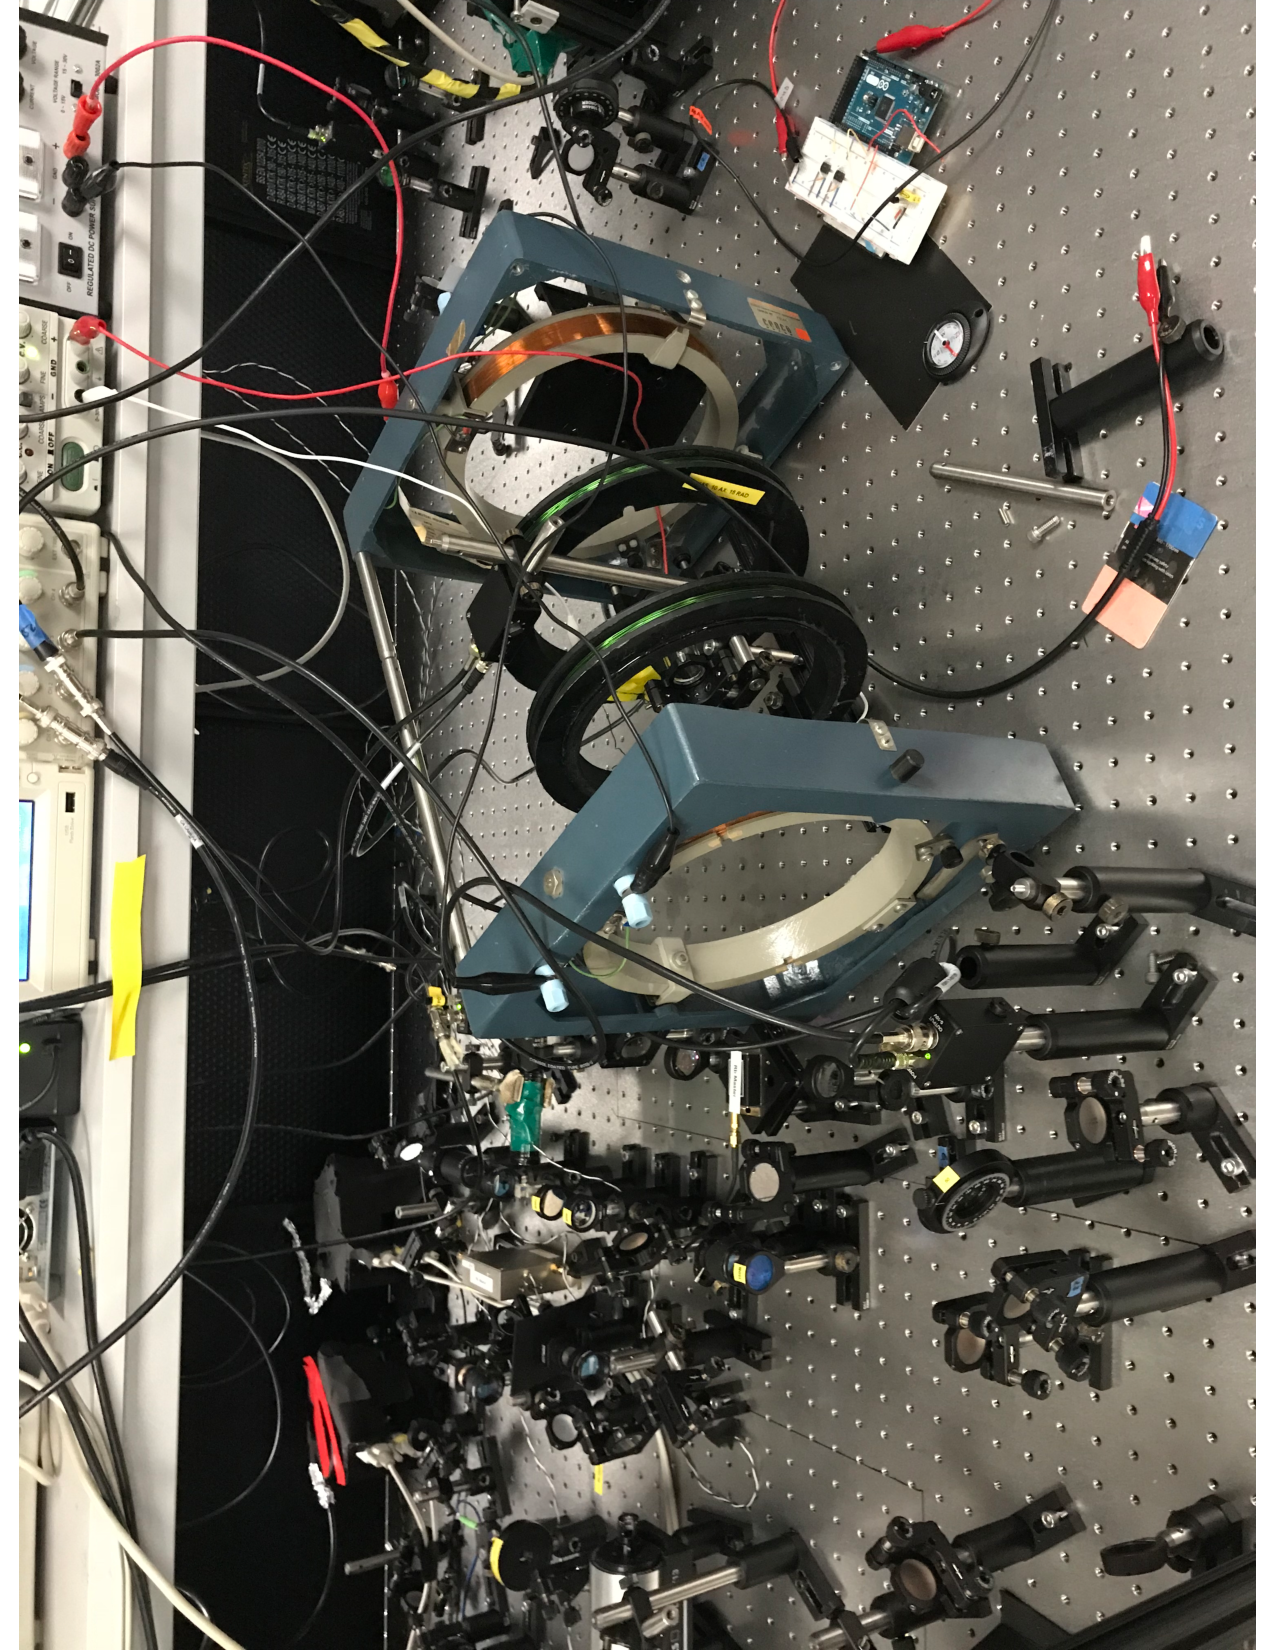
\includegraphics[width=0.8\textwidth]{Images/setup.png}};
		\node[text = white] at (1.5,-3) {\large Compensation};
		\node[text = white] at (.5,-3.5) {\large Coils};
		\node[text = white] at (2,-1.5) {\large Main};
		\node[text = white] at (2,-2.0) {\large Coils};
		\node[text = white] at (0,2) {\large Photodiode};
		\draw[red,->,stealth, line width = 1.6pt] (-2.5,-2.2) -- (-.5,-1.1);
		\node[text = white] at (-3,-1.5) {\large Laser};
	\end{tikzpicture}
	\caption{Experimental setup shown with compensation coils, main coils, absorption cell, and laser beam.}
	\label{fig:expsetupactual}
\end{figure}

The photodiodes were connected to an oscilloscope which was triggered at the scanning frequency of the diode laser. Fluorescence was measured by recording the potential difference from the oscilloscope, and was divided by the average power of the laser. This division is important as it allows us to compare the fluorescence between pulsed and continuous wave laser beams. Without it, the fluorescence from the continuous wave beam would consistently be greater since this beam has a higher average power.

%In order to characterize the fluorescence of rubidium from the constructed laser, a measurement of the saturation intensity of rubidium was taken. This is a measurement of the fluorescence of the atoms as a function of the average power of the laser, and indicates the power at which the atoms are being excited as quickly as possible. Above this intensity, no extra laser power will result in more atoms absorbing and emitting more light. This measurement was made with no magnetic field and the laser operating in continuous wave mode. These data are shown in Fig. \ref{fig:satint}. The error bars come from uncertainty in the fluorescence measurements recorded from the oscilloscope. A best best fit function,
%
%\begin{equation}
%	\text{f} = \frac{1}{1+e^{-1.6 \left( p - 1.1 \right) }},
%	\label{eq:satint}
%\end{equation}
%%
%where f is the fluorescence of the atoms and $p$ is the laser power in milliwatts.
%
%\begin{figure}[htpb]
%	\centering
%	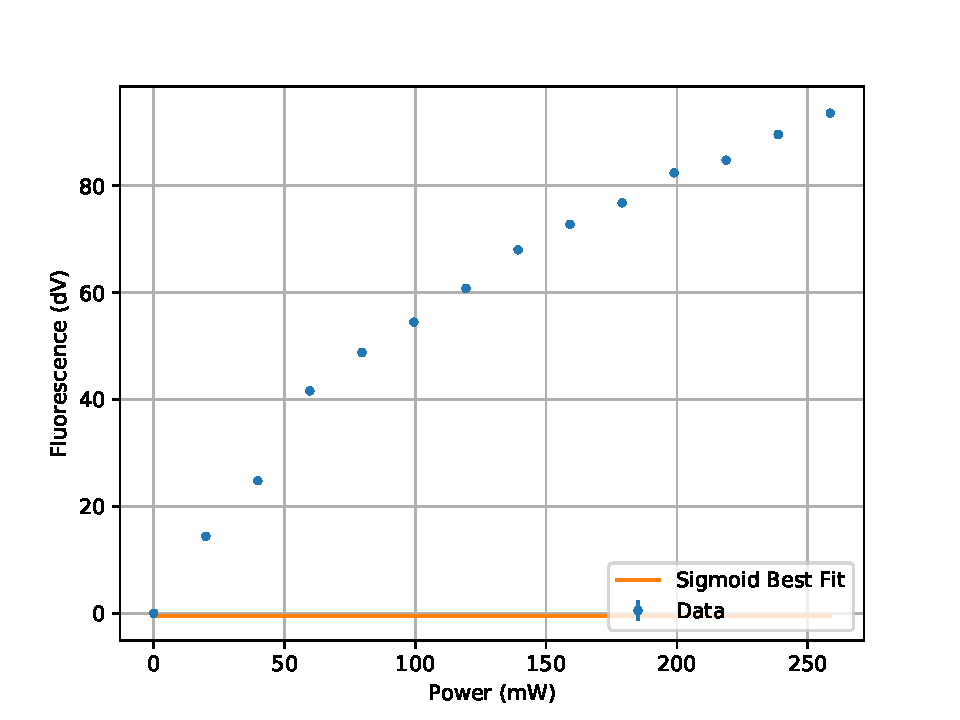
\includegraphics[width=0.8\textwidth]{../../Diode/SatCont.pdf}
%	\caption{Saturation intensity for rubidium pumped with the diode laser operating in continuous wave. A line of best fit is also plotted, given by Eq. \ref{eq:satint}. The error bars come from uncertainty in the fluorescence measurements.}
%	\label{fig:satint}
%\end{figure}



\section{Fluorescence versus Field and Repetition Rate}

The first measurement taken was of the fluorescence with respect to the magnetic field strength. With a magnetic field perpendicular to the laser beam and circularly polarized light, we performed this measurement to search for an increase in fluorescence when the repetition rate of the laser matched the Lamor frequency of the atoms. An arbitrary current was chosen (0.12 A), from this the magnetic field was calculated using Eq. \ref{eq:fieldvcurrent} (1.3 G), and then the Larmor frequency of rubidium in this magnetic field was calculated using Eq. \ref{zeemanf} (610 kHz). The repetition rate of the diode laser was set to this Larmor frequency using the function generator and the current was varied around the 0.12 A, thus changing the strength of the magnetic field. The expected result was an increase in the fluorescence around 0.12 A and this result was found. These data are shown in Fig. \ref{fig:flvc}, with a peak at \SI{0.12}{ A}. The error in the measurements comes from uncertainty in the potential difference read from the oscilloscope (which can be quite large, due to jitter in the laser and electronic noise) and from error in measuring the power of the laser beam.


\begin{figure}[htpb]
	\centering
	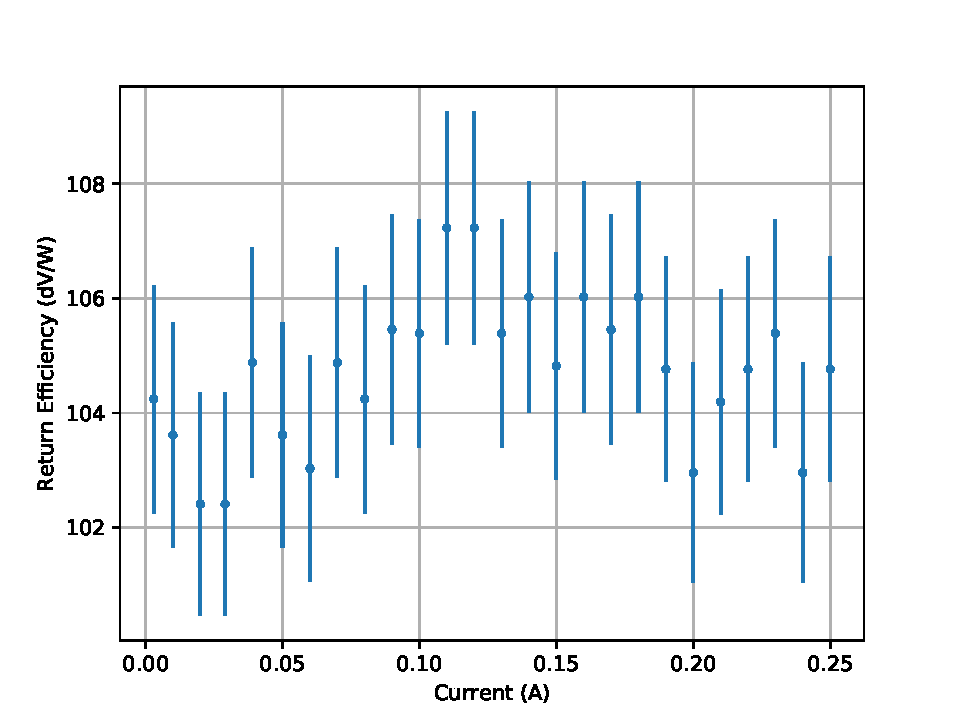
\includegraphics[width=0.8\textwidth]{../../MRPData/EfficiencyCurr.pdf}
	\caption{Fluorescence versus current with magnetic field perpendicular to laser beam and the repetition rate set at \SI{700}{ kHz}. The expected increase at 0.12 A is seen. The error in the measurements comes from uncertainty in the potential difference read from the oscilloscope (which can be quite large, due to jitter in the laser and electronic noise) and from error in measuring the power of the laser beam.}
	\label{fig:flvc}
\end{figure}

The second measurement taken was of fluorescence versus repetition rate with a constant magnetic field perpendicular to the laser beam. With the current set to 0.12 A (a magnetic field of \SI{1.3}{ G}), the expected peak in fluorescence would occur at \SI{700}{ kHz}. The fluorescence indeed peaked at \SI{700}{ kHz}, which can be seen in Fig. \ref{fig:flvrep}. The error comes from uncertainty in the fluorescence measurement as well as uncertainty in the average laser power measurement. Since, for magnetic fields perpendicular to the laser beam, the total angular momentum vector precesses in time about the axis of the field, optical pumping is not as efficient for this orientation as it is when the magnetic field is parallel to the beam. However, this confirmed that MRP can restore the benefits of optical pumping by only ``talking'' to the atoms at one point in their angular momentum's precession. We report a 14\% increase in fluorescence as the repetition rate of the laser is tuned to the Larmor frequency, with a full width at half-maximum of approximately \SI{50}{ kHz}.

\begin{figure}[ht]
	\centering
	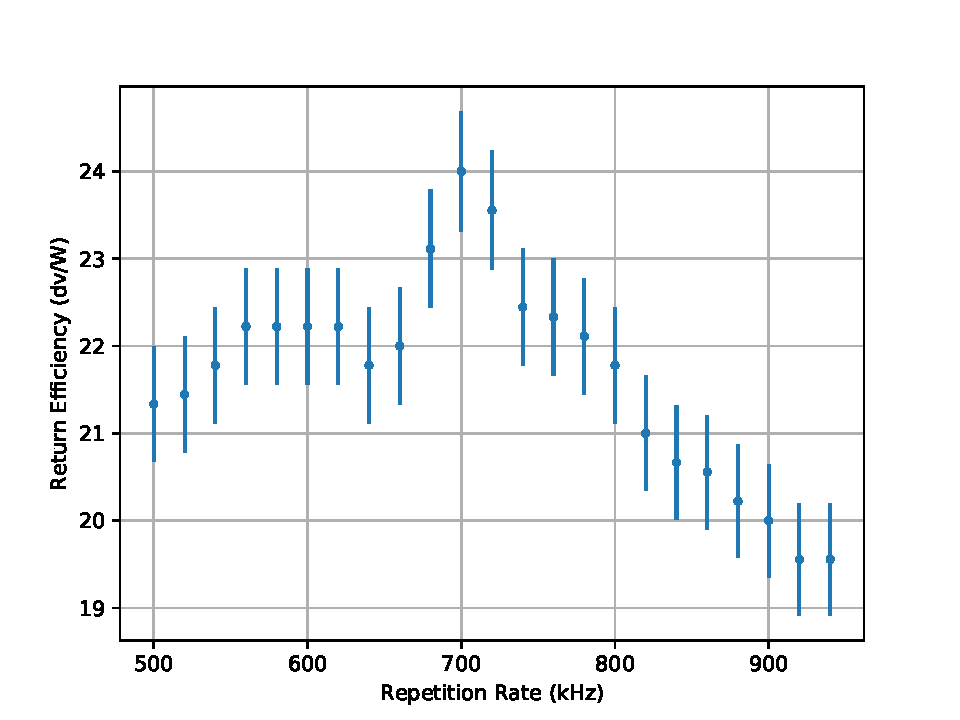
\includegraphics[width=0.8\textwidth]{../../MRPData/MAR24/FLvRep.pdf}
	\caption{Fluorescence of rubidium in a magnetic field of approximately 1.3 G perpendicular to laser beam as a function of repetition rate. The peak at \SI{700}{ kHz} shows the increase in fluorescence at the Larmor frequency of the atoms. The error comes from uncertainty in the fluorescence measurement as well as uncertainty in the average laser power measurement.}
	\label{fig:flvrep}
\end{figure}


\section{Fluorescence versus Angle}
We next took measurements of the fluorescence versus the angle between the magnetic field and the laser beam. Measurements were taken with the laser operating in pulsed and continuous wave mode, as well as with linearly and circularly polarized light. The magnetic field was tuned to the repetition rate such that the system was in MRP and there was a maximum in fluorescence. Fluorescence measurements were then recorded at various angles of the magnetic field with respect to the laser beam. A schematic of this is shown in Fig. \ref{fig:flvanglesch}. The results according to Kane et al. \cite{Kane2014} are as follows:

\begin{figure}[htpb]
	\centering
	\includestandalone[width=0.8\textwidth]{Images/tikz/FlvsAngle}
	\caption{Schematic of the rotation of the magnetic field with respect to laser beam.}
	\label{fig:flvanglesch}
\end{figure}


\begin{itemize}
	\item Circularly polarized light operating in pulsed and continuous mode give roughly equal fluorescence at $0^{\circ}$.
	\item As the angle between the magnetic field and laser beam increases, the fluorescence from circularly polarized, pulsed light stays constant while circularly polarized, continuous wave light decreases.
	\item The fluorescence from linearly polarized, continuous wave and linearly polarized, pulsed light should be lower than circularly polarized light, but should stay constant over all angles.
\end{itemize}

The data obtained from our measurements are shown in Fig. \ref{fig:flvangle}. To summarize, our data show the following:
\begin{itemize}
	\item Fluorescence from circularly polarized, pulsed light stays constant over all angles between the magnetic field and the laser beam. Fluorescence from circularly polarized, continuous wave light decreases as the angle increases. This is expected.
	\item The fluorescence from circularly polarized, pulsed light and circularly polarized, continuous wave light is not equal at $0^{\circ}$. Circularly polarized, continuous wave light has the lowest fluorescence overall. This is not expected.
	\item The fluorescence from linearly polarized, pulsed and continuous wave light stays roughly constant over all angles. This is expected.
\end{itemize}

The most important aspect of these data is the different trends seen in the fluorescence from the circularly polarized, continuous wave light and the circularly polarized, pulsed light. For circularly polarized, continuous wave light, the fluorescence should decrease with increasing angle since the magnetic field at increasing angles is redistributing the total angular momentum of the atoms, degrading the benefits of optical pumping to be obtained. However, with pulsed light, the atoms are only being pumped at one point in their precession cycle. To the light, the atom seems to not be precessing at all, and the benefits of optical pumping are restored. Thus, for all angles, the fluorescence from the circularly polarized, pulsed light should stay constant, which it does.

There are, however, a few concerns with these data. Firstly, the fluorescence from circularly polarized, continuous wave and pulsed light is not equal at $0^{\circ}$. Secondly, circularly polarized, continuous wave light should result in higher fluorescence than linearly polarized, continuous wave light (this is optical pumping, described in Chapter 2), which these data do not show. It is possible that these problems are results of the intensity of the continuous wave light, which was found to be classified in a high intensity regime \cite{Kane2014}. At these intensities, transition saturation (one of the ``three evils'' of LGS; also known as depumping) becomes a  problem. Transition saturation is the decay of atoms to a lower ground state (the second hyperfine ground state) after emission of a photon. Atoms in this lower ground state cannot be excited by our laser since this transition requires a different wavelength for excitation. For high intensities, a significant number of atoms can decay into this lower ground state since atoms are being excited as rapidly as possible. This results in less atoms that can absorb and emit light, thereby decreasing the overall fluorescence (this is described more in the follow section). To mitigate the consequences of transition saturation, data were taken with CW light at a lower intensity (a power of around \SI{1}{\milli \watt}). These data, shown in Fig. \ref{fig:flvangle2}, show the correct vertical positions that are expected as well as the same trends seen in the previous data. 


\begin{figure}[htb]
	\centering
	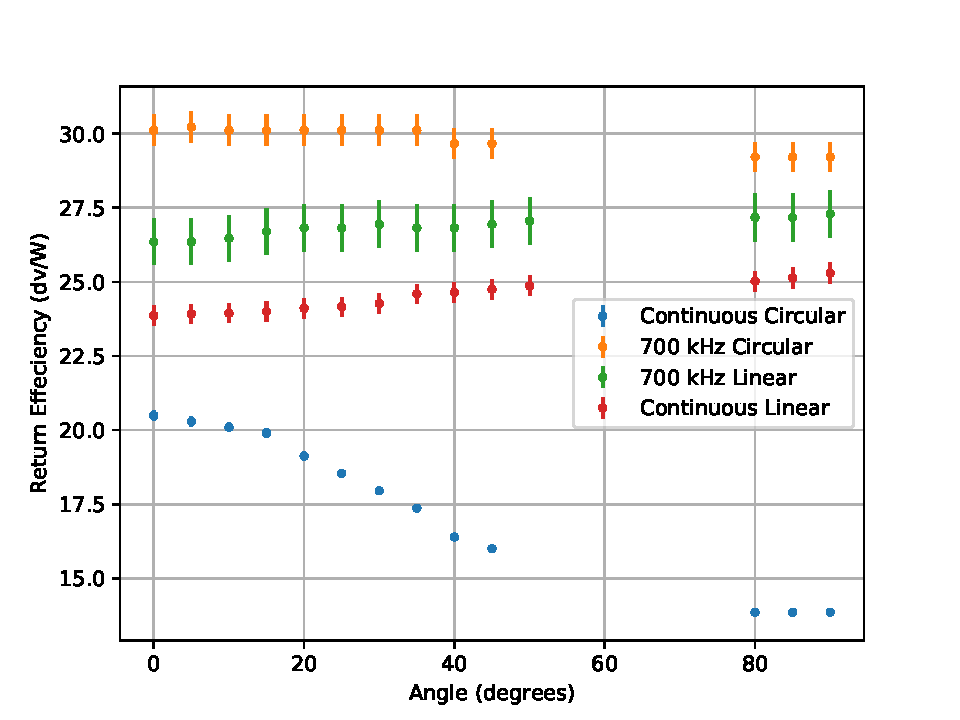
\includegraphics[width=0.8\textwidth]{../../MRPData/MAR24/together.pdf}
	\caption{Fluorescence of rubidium atoms in a magnetic field of approximately 1.3 Gauss as a function of the angle between the field and the laser beam in the high intensity case. Data of pulsed and continuous laser light circularly and linearly polarized are shown. Circularly polarized light with a repetition rate equal to the Larmor frequency gives the highest return for all magnetic field orientations.}
	\label{fig:flvangle}
\end{figure}

\begin{figure}[htb]
	\centering
	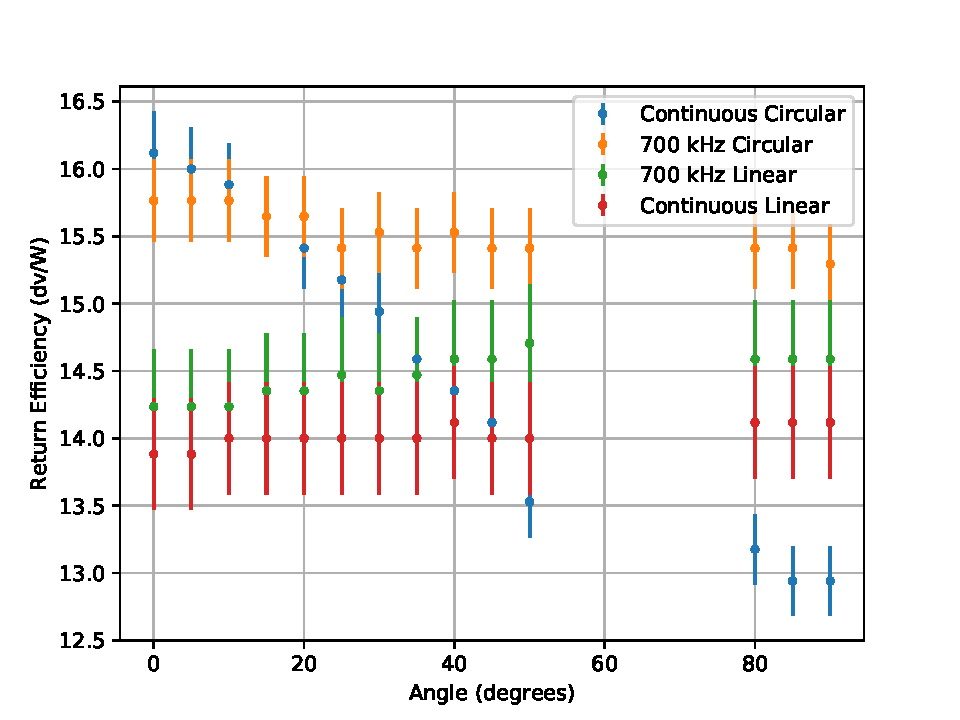
\includegraphics[width=0.8\textwidth]{../../MRPData/April16/together.pdf}
	\caption{Fluorescence of rubidium atoms in a magnetic field of approximately a few Gauss as a function of the angle between the field and the laser beam in the low intensity case. Data of pulsed and continuous laser light circularly and linearly polarized are shown. Circularly polarized light with a repetition rate equal to the Larmor frequency gives the highest return for all magnetic field orientations.}
	\label{fig:flvangle2}
\end{figure}

In order to look at overall trends and to better visualize the changes in fluorescence with increasing angle, we calculate the percent changes from maximum fluorescence, and plot them as well in Fig. \ref{fig:flvanglescaled}. We report a 33\% decrease in fluorescence for continuous wave, circularly polarized laser beams and a 2\% decrease in fluorescence for MRP laser beams at an angle of $90 \degrees$ between the laser beam and the magnetic field.

\begin{figure}[htb]
	\centering
	\begin{minipage}{.48\textwidth}
	\centering
		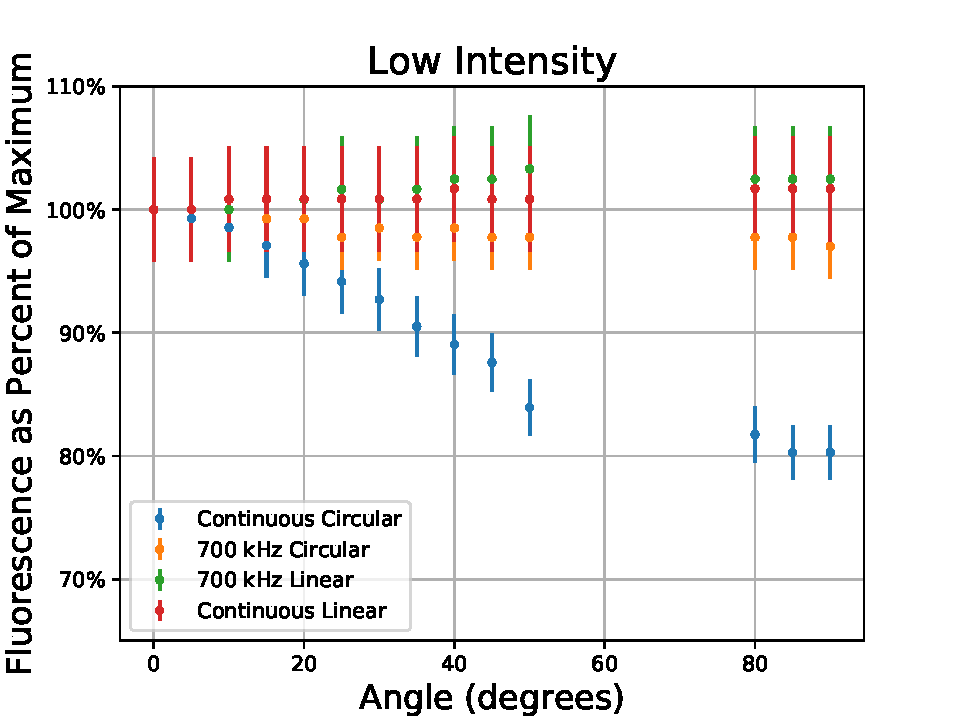
\includegraphics[width=0.9\textwidth]{../../MRPData/April16/togetherscaled.pdf}
	\end{minipage}
	\begin{minipage}{.48\textwidth}
	\centering
		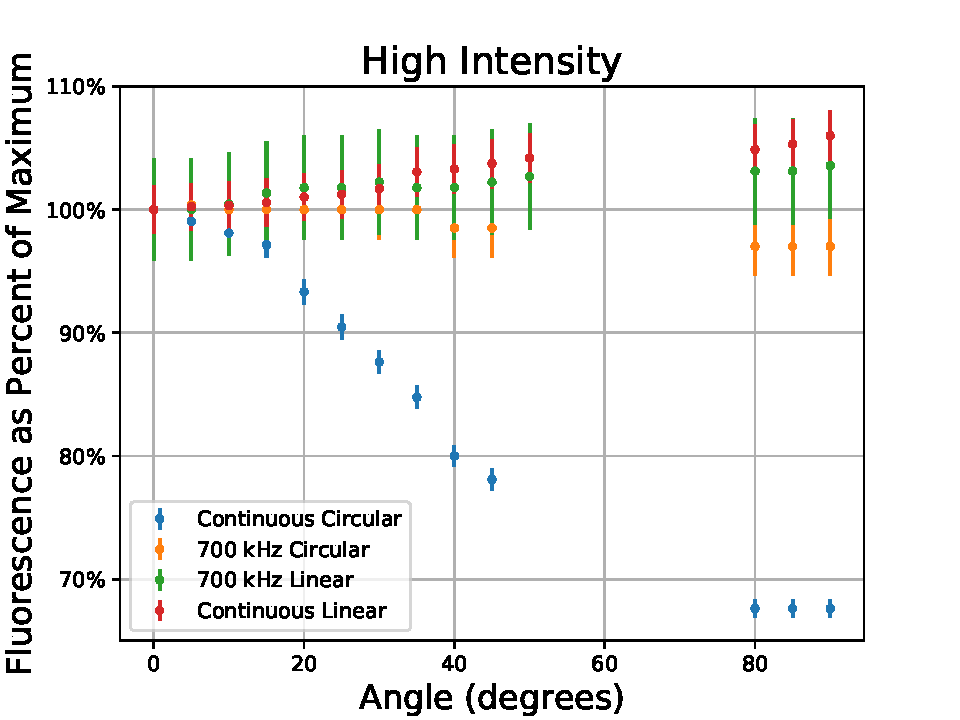
\includegraphics[width=0.9\textwidth]{../../MRPData/MAR24/togetherscaled.pdf}
	\end{minipage}
	\caption{Percent changes in fluorescence with respect to the maximum of rubidium atoms in a magnetic field of approximately 1.3 G as a function of the angle between the field and the laser beam. The low intensity case is shown on the left and the high intensity case shown on the right. Data of pulsed and continuous laser light circularly and linearly polarized are shown. Circularly polarized light with a repetition rate equal to the Larmor frequency gives the highest return for all magnetic field orientations.}
	\label{fig:flvanglescaled}
\end{figure}

\subsection{Repumping}
The transition we have been looking at so far is the $D_{2}$ transition, which is an excitation from the F = 2 to the excited state. As mentioned earlier and described in other papers \cite{Kane2014}, it is possible for atoms to decay into the lower ground state, F = 1, which cannot be accessed by our laser. This results in atoms falling into a dark state, causing an overall decrease in fluorescence. Thus, we introduced a repumper laser capable of accessing this transition. This would allow atoms in the second hyperfine ground state to be excited, thereby allowing that atom to contribute to the overall fluorescence. We theorized that the addition of this repumper would correct the incorrect vertical scale for circularly polarized, continuous wave light, seen in Fig \ref{fig:flvangle}. 

The repumper consisted of the same diode laser as described Section 3.2. However, the diffraction grating for this laser has a slightly different angle than the main laser, thus changing its wavelength enough to access the excitation from the second hyperfine ground state. The repumper beam was overlapped with the main laser beam using a polarizing beam splitting cube. This resulted in the repumper beam having linear polarization orthogonal to the main laser beam polarization. This results in the repumper beam having $\sigma^{-}$ circular polarization after linear to circular polarization conversion. As mentioned earlier, the main laser has $\sigma^{+}$ circular polarization.

We measured the fluorescence as $0^{\circ}$ and at $90^{\circ}$ between the laser and magnetic field for varying levels of repumper laser power. The fluorescence measurements were taken with three different levels of repumper percentages (rempumper power divided by main laser power): 0\%, 10\%, and 20\%. The data of these three levels are shown in Fig. \ref{fig:0repump}. We did not find the addition of the repumper to increase fluorescence for the pulsed laser. Instead, we found the opposite to be true! As repumper percentage increases, the fluorescence from the pulsed laser \textit{decreases} significantly.

\begin{figure}[htpb]
	\centering
	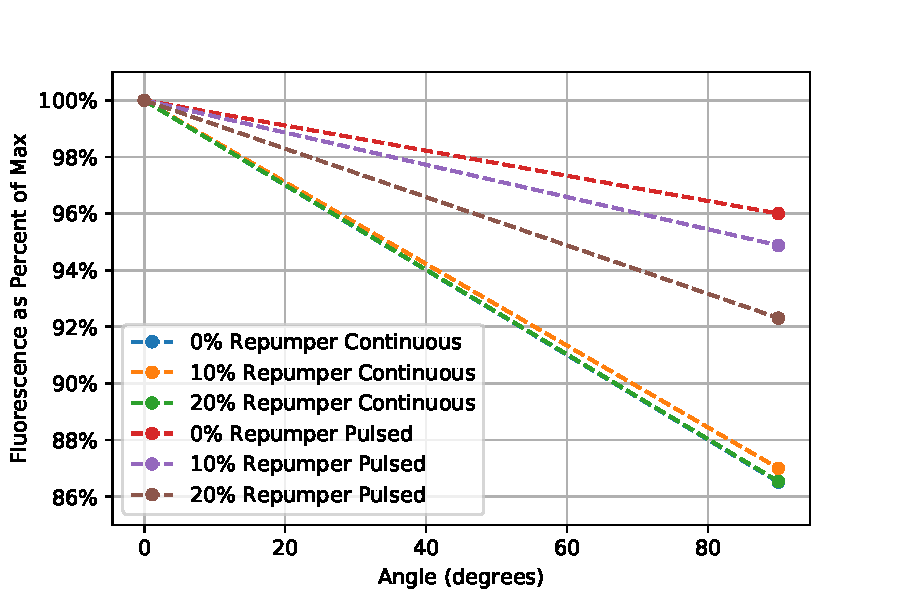
\includegraphics[width=0.9\textwidth]{../../MRPData/Repumping/20scaled.pdf}
	\caption{Fluorescence as percentage of maximum fluorescence versus the angle between the laser beam and magnetic field is shown for repumper percentages of 0\%, 10\%, and 20\%. The dashed lines do not constitute data but are shown to guide the eye.}
	\label{fig:0repump}
\end{figure}


We believe this trend to be true because of the polarization and CW mode of the repumper. The repumper has $\sigma^{-}$ circular polarization, which pushes atoms into lower angular momentum states as opposed to the main laser, which pushed atoms into higher angular momentum states. We can quickly and \textit{roughly} estimate if this is significant or not. The main laser has a repetition rate of \SI{700}{\kilo Hz} and a duty cycle of 20\%. Thus, each pulse width is about \SI{0.28}{\micro \second}. In this time, a cycling transition needs to be established. Since the  repumper is on all the time (continuous wave), it has a very large amount of time (compared to the main pulsed laser) to push atoms into the lowest angular momentum state, $m_F = -4$. Then as the main laser pumps the atoms, it will take roughly 10 transitions to get to the cycling transition of highest angular momentum (there are only 7 transitions, but each transition has roughly a 1/3 probability\footnote{The probability is actually not 1/3, nor do the transitions have the same probability. We use a 1/3 probability in order to get a rough estimate. See Steck (2001) for more information on decay rates \cite{steck}.} of decaying into a lower angular momentum state). The life time of an excited state is \SI{1.6e-8}{\second} \cite{steck}. Thus, it will take \SI{0.26}{\micro \second} to reach a cycling transition. However, this is roughly the pulse width, so in the time that it takes the atoms to get into the cycling transition, the pulse has ended and the repumper pushes the atoms back down to the lowest angular momentum state, undoing the whole effort. Thus, the cycling transition cannot be maintained. Going forward, the repumper should be pulsed along with the main laser so that it is only acting in conjunction with the main laser. Furthermore, the repumper should have the same polarization as the main laser so that it does not push atoms down to lower angular momentum states but instead pushes atoms towards higher angular momentum states where a cycling transition can be established.

Lastly, we wanted to fix some of the problems we found with the first fluorescence versus angle data taken, shown in Fig. \ref{fig:flvangle}. It was seen that the fluorescence from the circularly polarized, continuous wave light was significantly lower than the fluorescence from the circularly polarized, pulsed light, which was not expected. We thought that this might be due to the transition saturation, and theorized that a repumper would fix this problem. We thus retook this data for circularly polarized, pulsed light at \SI{1.5}{\milli W}, circular continuous light at \SI{6}{\milli W} without a repumper, and circular continuous light at \SI{6}{\milli W} with 20\% repumper. These data are shown in Fig. \ref{fig:flvanglerepump}, and it is seen that the repumper indeed increases fluorescence to the proper vertical position. This confirmed that transition saturation was occurring for laser beams with high intensity in our data.

\begin{figure}[htpb]
	\centering
	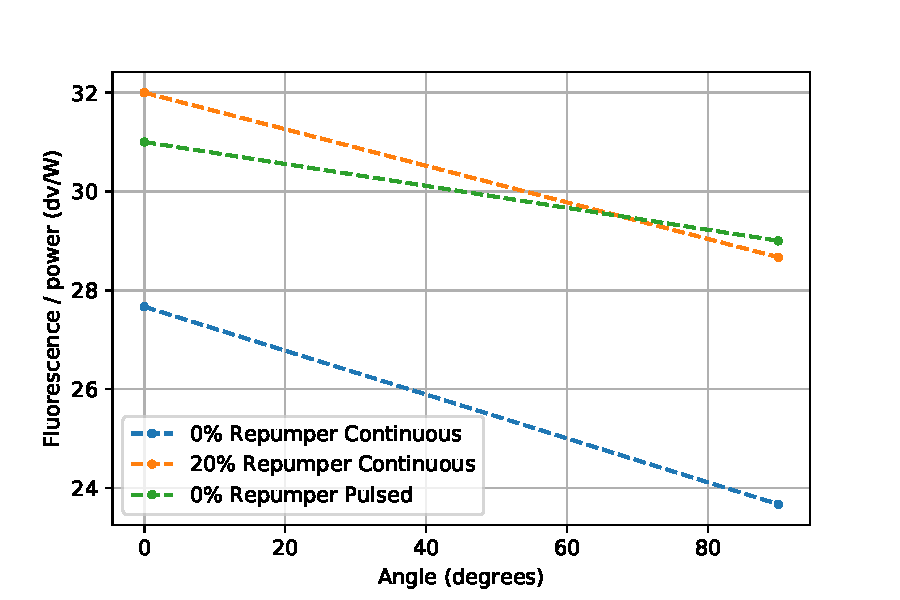
\includegraphics[width=0.8\textwidth]{../../MRPData/Repumping/transat.pdf}
	\caption{Fluorescence versus angle for circular pulsed light, circular continuous light, and circular continuous light with the repumper.}
	\label{fig:flvanglerepump}
\end{figure}

\subsection{Backscatter Fluorescence}
All of the previous data were measured using photodiode 1 (from top down) since this allowed the collection of light to not be interrupted with the rotation of the main coils. In order to ensure that backscatter fluorescence indeed followed these same trends (since telescopes rely on the backscattered light from laser guide stars), we took two data points, at $0^{\circ}$ and $90^{\circ}$ measured with photodiode 2 (backscatter). Only two data points were taken because, for many angles, the main coils were in between the rubidium cell and the photodiode. These data confirm that MRP behaves similarly when measuring backscatter. These data are shown in Fig. \ref{fig:backscatter} as the raw data and as percentage changes from maximum fluorescence. The backscatter fluorescence was shown to decrease by nearly 18\% for a change in angle from $0^{\circ}$ to $90^{\circ}$.

\begin{figure}[htb]
	\centering
	\begin{minipage}{.49\textwidth}
	\centering
		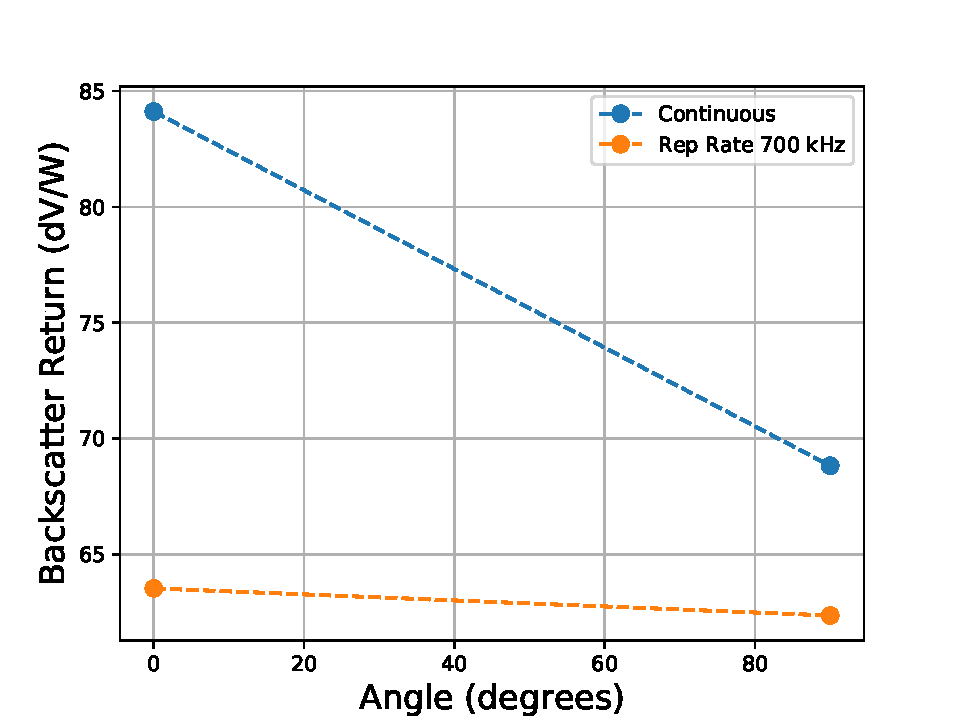
\includegraphics[width=0.9\textwidth]{../../MRPData/Backscatter/backscatter.pdf}
	\end{minipage}
	\begin{minipage}{.49\textwidth}
	\centering
		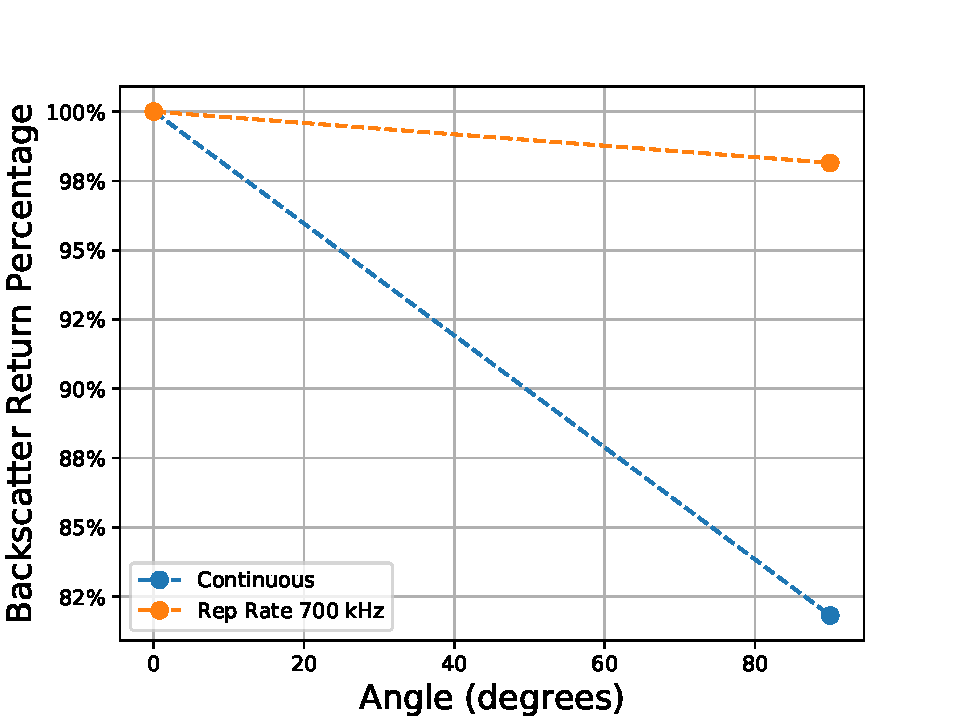
\includegraphics[width=0.9\textwidth]{../../MRPData/Backscatter/backscatterScaled.pdf}
	\end{minipage}
	\caption{Fluorescence for circularly polarized light with continuous light and pulsed light at the Larmor frequency; raw data is shown on the left and percent changes from maximum fluorescence data on the right. It is seen that backscatter agrees well with the data taken from top down. The dashed lines do not constitute data but are shown to guide the eye.}
	\label{fig:backscatter}
\end{figure}


